\documentclass[journal=asbcd6,manuscript=article]{achemso}

\usepackage{natbib}
\usepackage{setspace}
\usepackage{xkeyval}
\usepackage{array}
\usepackage{listings}
\usepackage{lmodern}
\usepackage{mathpazo}
\usepackage{geometry}
\usepackage{microtype}
\usepackage{url}  % Formatting web addresses
\usepackage{ifthen}  % Conditional
\usepackage{multicol}   %Columns
\usepackage[utf8]{inputenc} %unicode support
\usepackage{amsmath}
\usepackage{amssymb}
\usepackage{mathtools}
\usepackage{epsfig}
\usepackage{epstopdf}
\usepackage{graphicx}
\usepackage{textcomp}
\usepackage{multirow}
\usepackage{booktabs}
\usepackage{natmove}
\usepackage{float}
\usepackage[margin=0.1pt,font=footnotesize,labelfont=bf]{caption}
\usepackage[version=3]{mhchem} % Formula subscripts using \ce{}
\usepackage[T1]{fontenc}       % Use modern font encodings
%\usepackage[square,sort,comma,numbers,sort&compress]{natbib}
%%%%%%%%%%%%%%%%%%%%%%%%%%%%%%%%%%%%%%%%%%%%%%%%%%%%%%%%%%%%%%%%%%%%%
%% If issues arise when submitting your manuscript, you may want to
%% un-comment the next line.  This provides information on the
%% version of every file you have used.
%%%%%%%%%%%%%%%%%%%%%%%%%%%%%%%%%%%%%%%%%%%%%%%%%%%%%%%%%%%%%%%%%%%%%
%%\listfiles

%\bibliographystyle{achemso}
\newcommand*\mycommand[1]{\texttt{\emph{#1}}}
%%%%%%%%%%%%%%%%%%%%%%%%%%%%%%%%%%%%%%%%%%%%%%%%%%%%%%%%%%%%%%%%%%%%%

%%%%%%%%%%%%%%%%%%%%%%%%%%%%%%%%%%%%%%%%%%%%%%%%%%%%%%%%%%%%%%%%%%%%%
\author{Michael Vilkhovoy}
\affiliation[Cornell University]
{Robert Frederick Smith School of Chemical and Biomolecular Engineering, Cornell University, Ithaca, NY 14853}
\author{Nicholas Horvath}
\affiliation[Cornell University]
{Robert Frederick Smith School of Chemical and Biomolecular Engineering, Cornell University, Ithaca, NY 14853}
\author{Joseph Wayman}
\affiliation[Cornell University]
{Robert Frederick Smith School of Chemical and Biomolecular Engineering, Cornell University, Ithaca, NY 14853}
\author{Kara Calhoun}
\affiliation[Stanford University]
{School of Chemical Engineering, Stanford University, Stanford, CA 94305}
\author{James Swartz}
\affiliation[Stanford University]
{School of Chemical Engineering, Stanford University, Stanford, CA 94305}
\author{Jeffrey D. Varner}
\email{jdv27@cornell.edu}
\phone{+1~(607)~255-4258}
\fax{+1~(607)~255-9166}
\affiliation[Cornell University]
{Robert Frederick Smith School of Chemical and Biomolecular Engineering, Cornell University, Ithaca, NY 14853}
%%%%%%%%%%%%%%%%%%%%%%%%%%%%%%%%%%%%%%%%%%%%%%%%%%%%%%%%%%%%%%%%%%%%%
\title{Sequence Specific Modeling of \emph{E.~coli} Cell-Free Protein Synthesis}
%\abbreviations{MV,NH,JDV}
\keywords{Synthetic biology, constraints based modeling, cell-free protein synthesis}

\begin{document}

%%%%%%%%%%%%%%%%%%%%%%%%%%%%%%%%%%%%%%%%%%%%%%%%%%%%%%%%%%%%%%%%%%%%%
%% The abstract environment will automatically gobble the contents
%% if an abstract is not used by the target journal.
%%%%%%%%%%%%%%%%%%%%%%%%%%%%%%%%%%%%%%%%%%%%%%%%%%%%%%%%%%%%%%%%%%%%%
\begin{abstract}
Cell-free protein expression has become a widely used research tool in systems and synthetic biology, and a promising technology for personalized medicine.
In this study, we used sequence specific constraint based modeling to evaluate the performance of an \emph{E.~coli} cell-free protein synthesis system.
A core \emph{E.~coli} metabolic model, describing glycolysis, the pentose phosphate pathway, amino acid biosynthesis and degradation and energy metabolism,
was augmented with sequence specific descriptions of transcription and translation processes, and effective models of promoter function.
Thus, sequence specific constraint based modeling explicitly couples transcription and translation processes, and the regulation of gene expression,
with the availability of metabolic resources.
We tested this approach by simulating the expression of two model proteins chloramphenicol acetyltransferase and dual emission green fluorescent protein for which we have training data sets;
we then expanded the simulations to a range of therapeutically relevant proteins.
Protein expression simulations were consistent with measurements for a variety of cases.
Further, global sensitivity analysis identified the key metabolic processes that controlled the productivity, energy efficiency, and carbon yield of the process.
Taken together, sequence specific constraint based modeling offers a novel means to \emph{a~priori} estimate the performance of cell-free synthetic circuits.
\end{abstract}

% A sufficient energy supply with oxidative phosphorylation is instrumental for high energy efficiency and carbon yields; in addition, the translation rate could be optimized for higher productivity.

%%%%%%%%%%%%%%%%%%%%%%%%%%%%%%%%%%%%%%%%%%%%%%%%%%%%%%%%%%%%%%%%%%%%%
%% Start the main part of the manuscript here.
%%%%%%%%%%%%%%%%%%%%%%%%%%%%%%%%%%%%%%%%%%%%%%%%%%%%%%%%%%%%%%%%%%%%%

\section{Introduction}
Cell-free protein expression has become a widely used research tool in systems and synthetic biology, and a promising technology for personalized protein production.
Cell-free systems offer many advantages for the study, manipulation and modeling of metabolism compared to \textit{in vivo} processes.
Central amongst these, is direct access to metabolites and the biosynthetic machinery without the interference of a cell wall, or complications associated with cell growth.
This allows us to interrogate the chemical environment while the biosynthetic machinery is operating, potentially at a fine time resolution.
Cell-free protein synthesis (CFPS) systems are arguably the most prominent examples of cell-free systems used today \cite{Jewett:2008aa}.
However, CFPS is not new; CFPS in crude \textit{E.~coli} extracts has been used since the 1960s to explore fundamental biological mechanisms \cite{MATTHAEI:1961aa,NIRENBERG:1961aa}.
Today, cell-free systems are used in a variety of applications ranging from therapeutic protein production \cite{Lu:2014aa} to synthetic biology \cite{Hodgman:2012aa}.
However, if CFPS is to become a mainstream technology for applications such as point of care manufacturing \cite{Pardee2016248}, we must first understand the performance limits and cost of these systems \cite{Jewett:2008aa}.
One tool to address these questions is mathematical modeling.

% Interestingly, many of the challenges confronting \textit{in~vivo} genome scale kinetic modeling can potentially be overcome in a cell-free system.
% For example, there is no complex transcriptional regulation to consider, transient metabolic measurements are easier to obtain, and we no longer have to consider cell growth.
% Thus, cell-free operation holds several significant advantages for model development, identification and validation.
% Theoretically, genome scale cell-free kinetic models may be possible for industrially important organisms, such as \textit{E.~coli} or \textit{B. subtilis}, if a simple, tractable framework for integrating allosteric regulation with enzyme kinetics can be formulated.
% Traditionally, stoichiometric models have also neglected explicit descriptions of metabolic regulation and control mechanisms, instead opting to describe the choice of pathways by prescribing an objective function on metabolism. Interestingly, similar to early cybernetic models, the most common metabolic objective function has been the optimization of biomass formation \cite{2002_ibarra_edwards_palsson_Nat}, although other metabolic objectives have also been estimated \cite{2007_schuetz_sauer_MolSysBio}.
% Recent advances in constraints based modeling have overcome the early shortcomings of the platform, including capturing metabolic regulation and control \cite{2013_hyduke_lewis_palsson_MolBioSys}. Thus, modern constraints based approaches are extremely useful for the discovery of metabolic engineering strategies and represent the state of the art in metabolic modeling \cite{2013_mccloskey_palsson_feist_MolSysBio, 2012_zomorrodi_maranas_MetaEng}.

Stoichiometric reconstructions of microbial metabolism, popularized by constraint based approaches such as flux balance analysis (FBA), have become standard tools to interrogate metabolism \cite{2012_lewis_palsson_NatRevMicrobio}.
Constraint based methods such as FBA, metabolic flux analysis (MFA) \cite{WIECHERT2001195}, and network decomposition approaches such as elementary modes \cite{Schuster:2000aa} or extreme pathways \cite{Schilling:2000aa} model intracellular metabolism using biochemical stoichiometry and other constraints such as thermodynamical feasibility \cite{Henry:2007,Hamilton:2013} under pseudo steady state conditions.
Constraint based approaches have predicted productivity \cite{Varma01101994, BTPR:BTPR2132}, yield \cite{Varma01101994}, mutant behavior \cite{Edwards2000}, and growth phenotypes \cite{Brien693} for biochemical networks of arbitrary complexity, including genome scale networks, using linear programming \cite{Covert:2004aa}.
Since the first genome scale stoichiometric model of \textit{E.~coli} \cite{2000_edwards_palsson_PNAS}, stoichiometric reconstructions of hundreds of organisms, including industrially important prokaryotes such as \textit{E.~coli} \cite{Feist:2007aa} or \textit{B. subtilis} \cite{Oh:2007aa}, are now available \cite{2009_feist_palsson_NatRevMicrobio}.
Stoichiometric reconstructions have been expanded to include the integration of metabolism with detailed descriptions of gene expression (ME-Model) \cite{Allen:2003aa, Brien693},
and protein structures (GEM-PRO) \cite{Zhang1544,Chang1220}.
These expansions have greatly increased the scope of questions these models can explore.
Constraint based methods are powerful tools to estimate the performance of metabolic networks with very few adjustable parameters.
However, constraint based methods are typically used to model \textit{in~vivo} processes, and have not yet been applied to cell-free metabolism.

In this study, we used sequence specific constraint based modeling to evaluate the performance of \emph{E.~coli} cell-free protein synthesis (CFPS).
A core \emph{E.~coli} cell-free metabolic model was developed from literature \cite{Feist:2007aa}.
This model, which described glycolysis, pentose phosphate pathway, amino acid biosynthesis and degradation and energy metabolism, was then augmented with
sequence specific descriptions of promoter function, transcription and translation processes.
Thus, sequence specific constraints based modeling explicitly coupled transcription and translation with the availability of metabolic resources.
We tested this approach by simulating the production of two model proteins, and then investigated the productivity, energy efficiency, and carbon yield for eight different proteins.
From this, higher carbon number proteins typically had lower productivity rates, energy efficiency, and carbon yields than that of the lower carbon number proteins.
Further, global sensitivity analysis identified the key metabolic processes that controlled circuit performance, showing oxidative phosphorylation as instrumental for maintaining a high energy efficiency and carbon yield and the translation rate for productivity.
Taken together, sequence specific constraints based modeling offers a novel means to \emph{a~priori} estimate the performance of cell-free synthetic circuits.

\clearpage

\section{Results and discussion}


% The goal of this work was first to construct a modeling framework to describe cell-free protein synthesis systems and to examine its performance in productivity, energy efficiency and carbon yield for a protein of interest.
% One mathematical framework that has found wide use in modeling metabolism is constraints based models such as flux balance analysis (FBA).
% FBA can predict how cells utilize nutrients to produce products by using the biochemical stoichiometry and thermodynamical feasibility under pseudo steady-state conditions.
% Traditionally, FBA is used to model \textit{in~vivo} processes; however, cell-free systems do not have growth associated reactions or transport through the cell membrane.
% Thus,
% sequence specific flux balance analysis (ssFBA) with a detailed promoter model  to examine the performance of CFPS.
% We first validated the ssFBA approach by comparing simulated and measured concentrations of two proteins from two

\subsection{Model derivation and validation}
The cell-free stoichiometric network was constructed by removing growth associated reactions from the \textit{i}AF1260 reconstruction of K-12 MG1655 \textit{E.~coli} \cite{Feist:2007aa},
and adding deletions associated with the specific cell-free system (see materials and methods).
We then added the transcription and translation template reactions of Allen and Palsson for the specific proteins of interest \cite{Allen:2003aa}.
A schematic of the metabolic network, which consisted of 264 reactions and 146 species, is shown in Fig.~\ref{fig:network}A.
The network described the major carbon and energy pathways, as well as amino acid biosynthesis and degradation pathways.
Using this network, in combination with effective promoter models taken from Moon et al. \cite{Moon:2012ab}, and literature values for cell-free culture parameters (Table ~\ref{tbl:parameters}),
we simulated the sequence specific production of two model proteins, chloramphenicol acetyltransferase (CAT) and dual emission green fluorescent protein (deGFP) using
different \textit{E.~coli} cell-free extracts.
The cell-free metabolic network, along with all model code and parameters, can be downloaded under an MIT software license from the Varnerlab website \cite{varnerlab}.

Cell-free simulations of the time evolution of CAT and deGFP production were consistent with experimental measurements (Fig. ~\ref{fig:network}B and C).
Chloramphenicol acetyltransferase (CAT), was produced under a T7 promoter in a glucose/NMP cell-free system \cite{2005_calhoun_BiotechnologyProgress}
using glucose as a carbon and energy source (Fig.~\ref{fig:network}B).
With the exception of the first 10-15 min, the cell-free prediction of CAT abundance was consistent with the measured values (coefficient of determination, R\textsuperscript{2} = 0.86).
On the other hand, deGFP was produced under a P70a promoter in TXTL 2.0 \textit{E.~coli} extract for eight hours using maltose as a carbon and energy source (Fig.~\ref{fig:network}C).
The cell-free simulation captured the overall trend of deGFP abundance, but failed to capture saturation at the end of the CFPS culture (R\textsuperscript{2} = 0.84).
Uncertainty in experimental factors such as the concentration of RNA polymerase, ribosomes,
transcription and translation elongation rates or the upper bounds for oxygen and glucose consumption rates (modeled as being normally distributed around the parameter values shown in Table ~\ref{tbl:parameters})
did not qualitatively alter the performance of the model (blue region, 95\% confidence estimate).
Together, these simulations suggested the description of transcription and translation, and its integration with metabolism encoded in the cell-free metabolic model, were consistent with experimental measurements.
However, these simulations were conducted at a single plasmid concentration of 5 nM.
Thus, it was unclear if the model could capture cell-free protein synthesis for a range of plasmid concentrations.

\begin{figure}[t!]
\centering
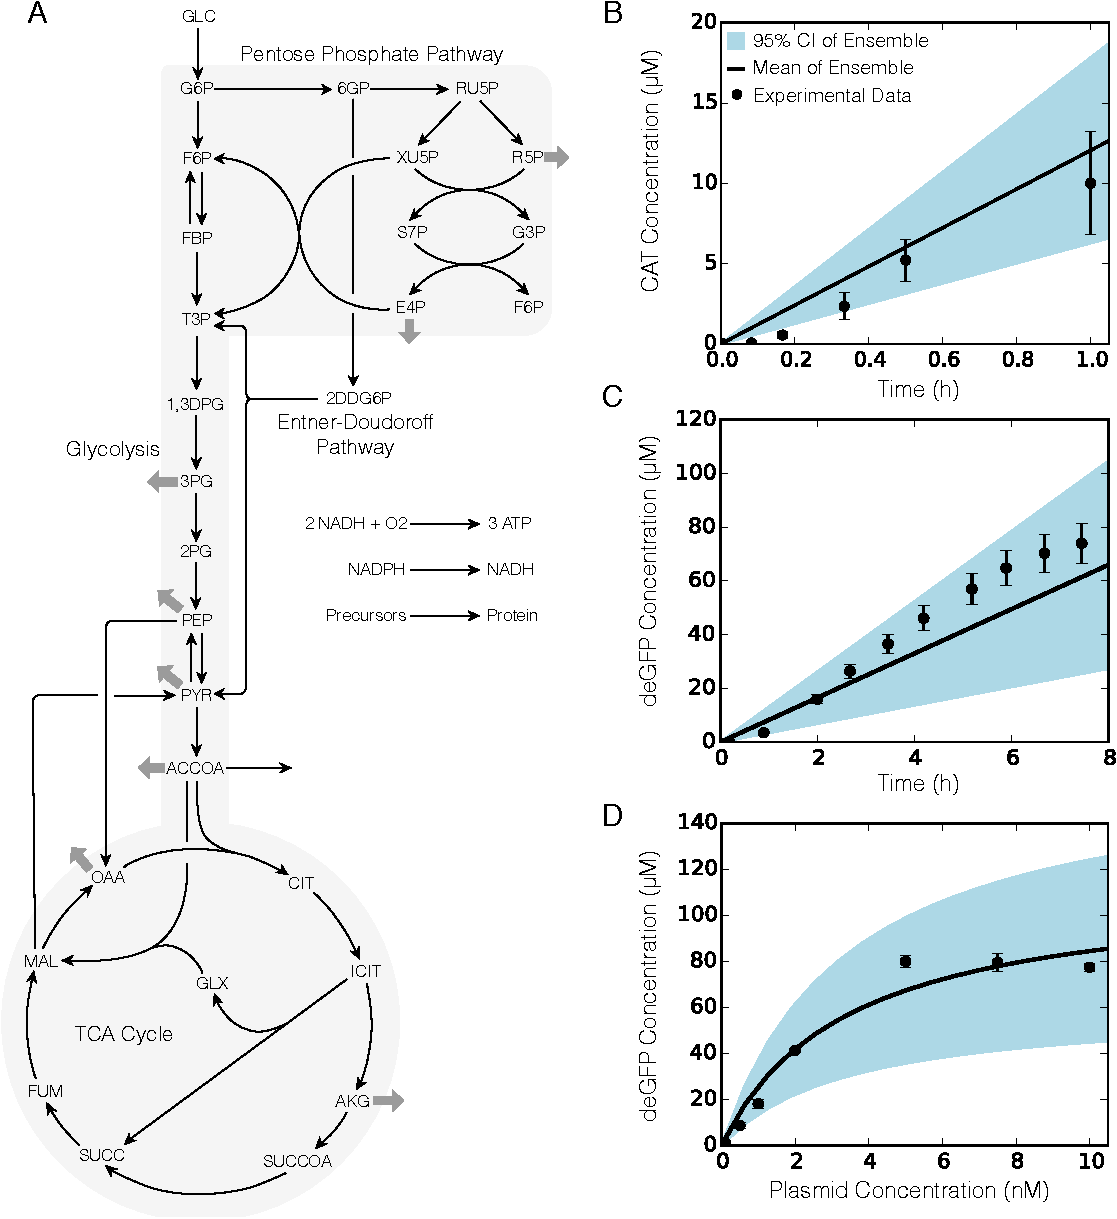
\includegraphics[width=1.00\textwidth]{./figs/Fig-1-Network-Validation-Simulations.pdf}
\caption{Sequence specific flux balance analysis. A. Core metabolic network with glycolysis, pentose phoshate pathway, TCA cycle, Entner-Doudoroff pathway. Thick gray arrows indicate withdrawal of precursors for amino acid synthesis. B. CAT production under a T7 promoter in CFPS \textit{E.~coli} extract for 1 h under glucose consumption. Error bars denote the standard deviation of experimental measurements. C. deGFP production under a P70 promoter in TXTL 2.0 \textit{E.~coli} extract for 8 h under maltose consumption. Error bars denote a 10\% coefficient of variation. D. Predicted deGFP concentration at different plasmid concentrations versus measurements of deGFP synthesized in TXTL 2.0. 95\% CI (blue region) over the ensemble of 100 sets, mean of the ensemble (black line), and experimental measurements (dots).}
\label{fig:network}
\end{figure}

Cell-free simulations of the deGFP titer for a range of plasmid concentrations were consistent with experimental measurements (Fig.~\ref{fig:network}D).
The cell-free deGFP titer at each plasmid concentration was calculated by multiplying the flux of deGFP synthesis by the active time of production, approximately 8 hours in TXTL 2.0 \cite{Garamella:2016aa}.
The mean of the ensemble (calculated by sampling the uncertainty in the model parameters) captured the saturation of deGFP production as a function of plasmid concentration  (R\textsuperscript{2} = 0.97).
However, while the mean and 95\% confidence estimate of the ensemble were consistent with measured deGFP levels, the model under predicted the deGFP titer at the saturating point of 5 nM of plasmid concentration.
These results, in combination with the time-dependent CAT and deGFP simulations, validated our CFPS modeling approach which required very few adjustable parameters.
It also showed that the sequence specific template reactions and metabolic network were sufficient to predict the production of different proteins under different promoters, and cell-free systems.
Next, we used our modeling approach to better understand the theoretical performance limits of CFPS.

%These amino acid synthesis reactions were blocked since during the cell-free extract preparation the cells are often supplied with amino acids; thus, the enzymes responsible for amino acid synthesis would not be present.
% We used ssFBA to estimate the productivity, energy efficiency, and carbon yield for each of these proteins for each case.

\subsection{Analysis of CFPS performance}
To better understand the performance of CFPS reactions, we predicted the productivity, energy efficiency and carbon yield for the cell-free production of eight model proteins with and without amino acid supplementation (Fig. \ref{fig:Prof}).
The expression of each of these proteins was under a P70a promoter, with the exception of CAT which was expressed using a T7 promoter.
In all cases, the CFPS reaction was supplied with glucose; however, we considered different scenarios for amino acid supplementation.
First, the CFPS reaction was supplied with amino acids, and simultaneously was also allowed to synthesize amino acids from glucose (AAs supplied and \textit{de~novo} synthesis).
Next, the CFPS reaction was supplied with both glucose and amino acids, but \textit{de~novo} amino acid biosynthesis was not allowed (AAs supplied w/o \textit{de~novo} synthesis).
This scenario was consistent with common cell-free extract preparation protocols which often involve amino acid supplementation;
thus, we expect the enzymes responsible for amino acid biosynthesis to be largely absent from the CFPS reaction in these cases.
Lastly, the cell-free reaction was given glucose but not supplemented with amino acids, and was forced to synthesize them \textit{de~novo} from glucose (\textit{de~novo} synthesis only).
Eight proteins, ranging in size, were selected to evaluate CFPS performance: bone morphogenetic protein 10 (BMP10),
chloramphenicol acetyltransferase (CAT), caspase 9 (CASP9), dual emission green fluorescent protein (deGFP),
prothrombin (FII), coagulation factor X (FX), fibroblast growth factor 21 (FGF21), and single chain variable fragment R4 (scFvR4).
An additional case was considered for CAT, where central metabolic fluxes were constrained by experimental metabolic measurements of glucose, organic and amino acid consumption/production rates (see supplemental materials).
Finally, we considered maltose binding protein (MBP) as a first principle prediction against the trends formulated by the other proteins.

\begin{figure}[t!]
\centering
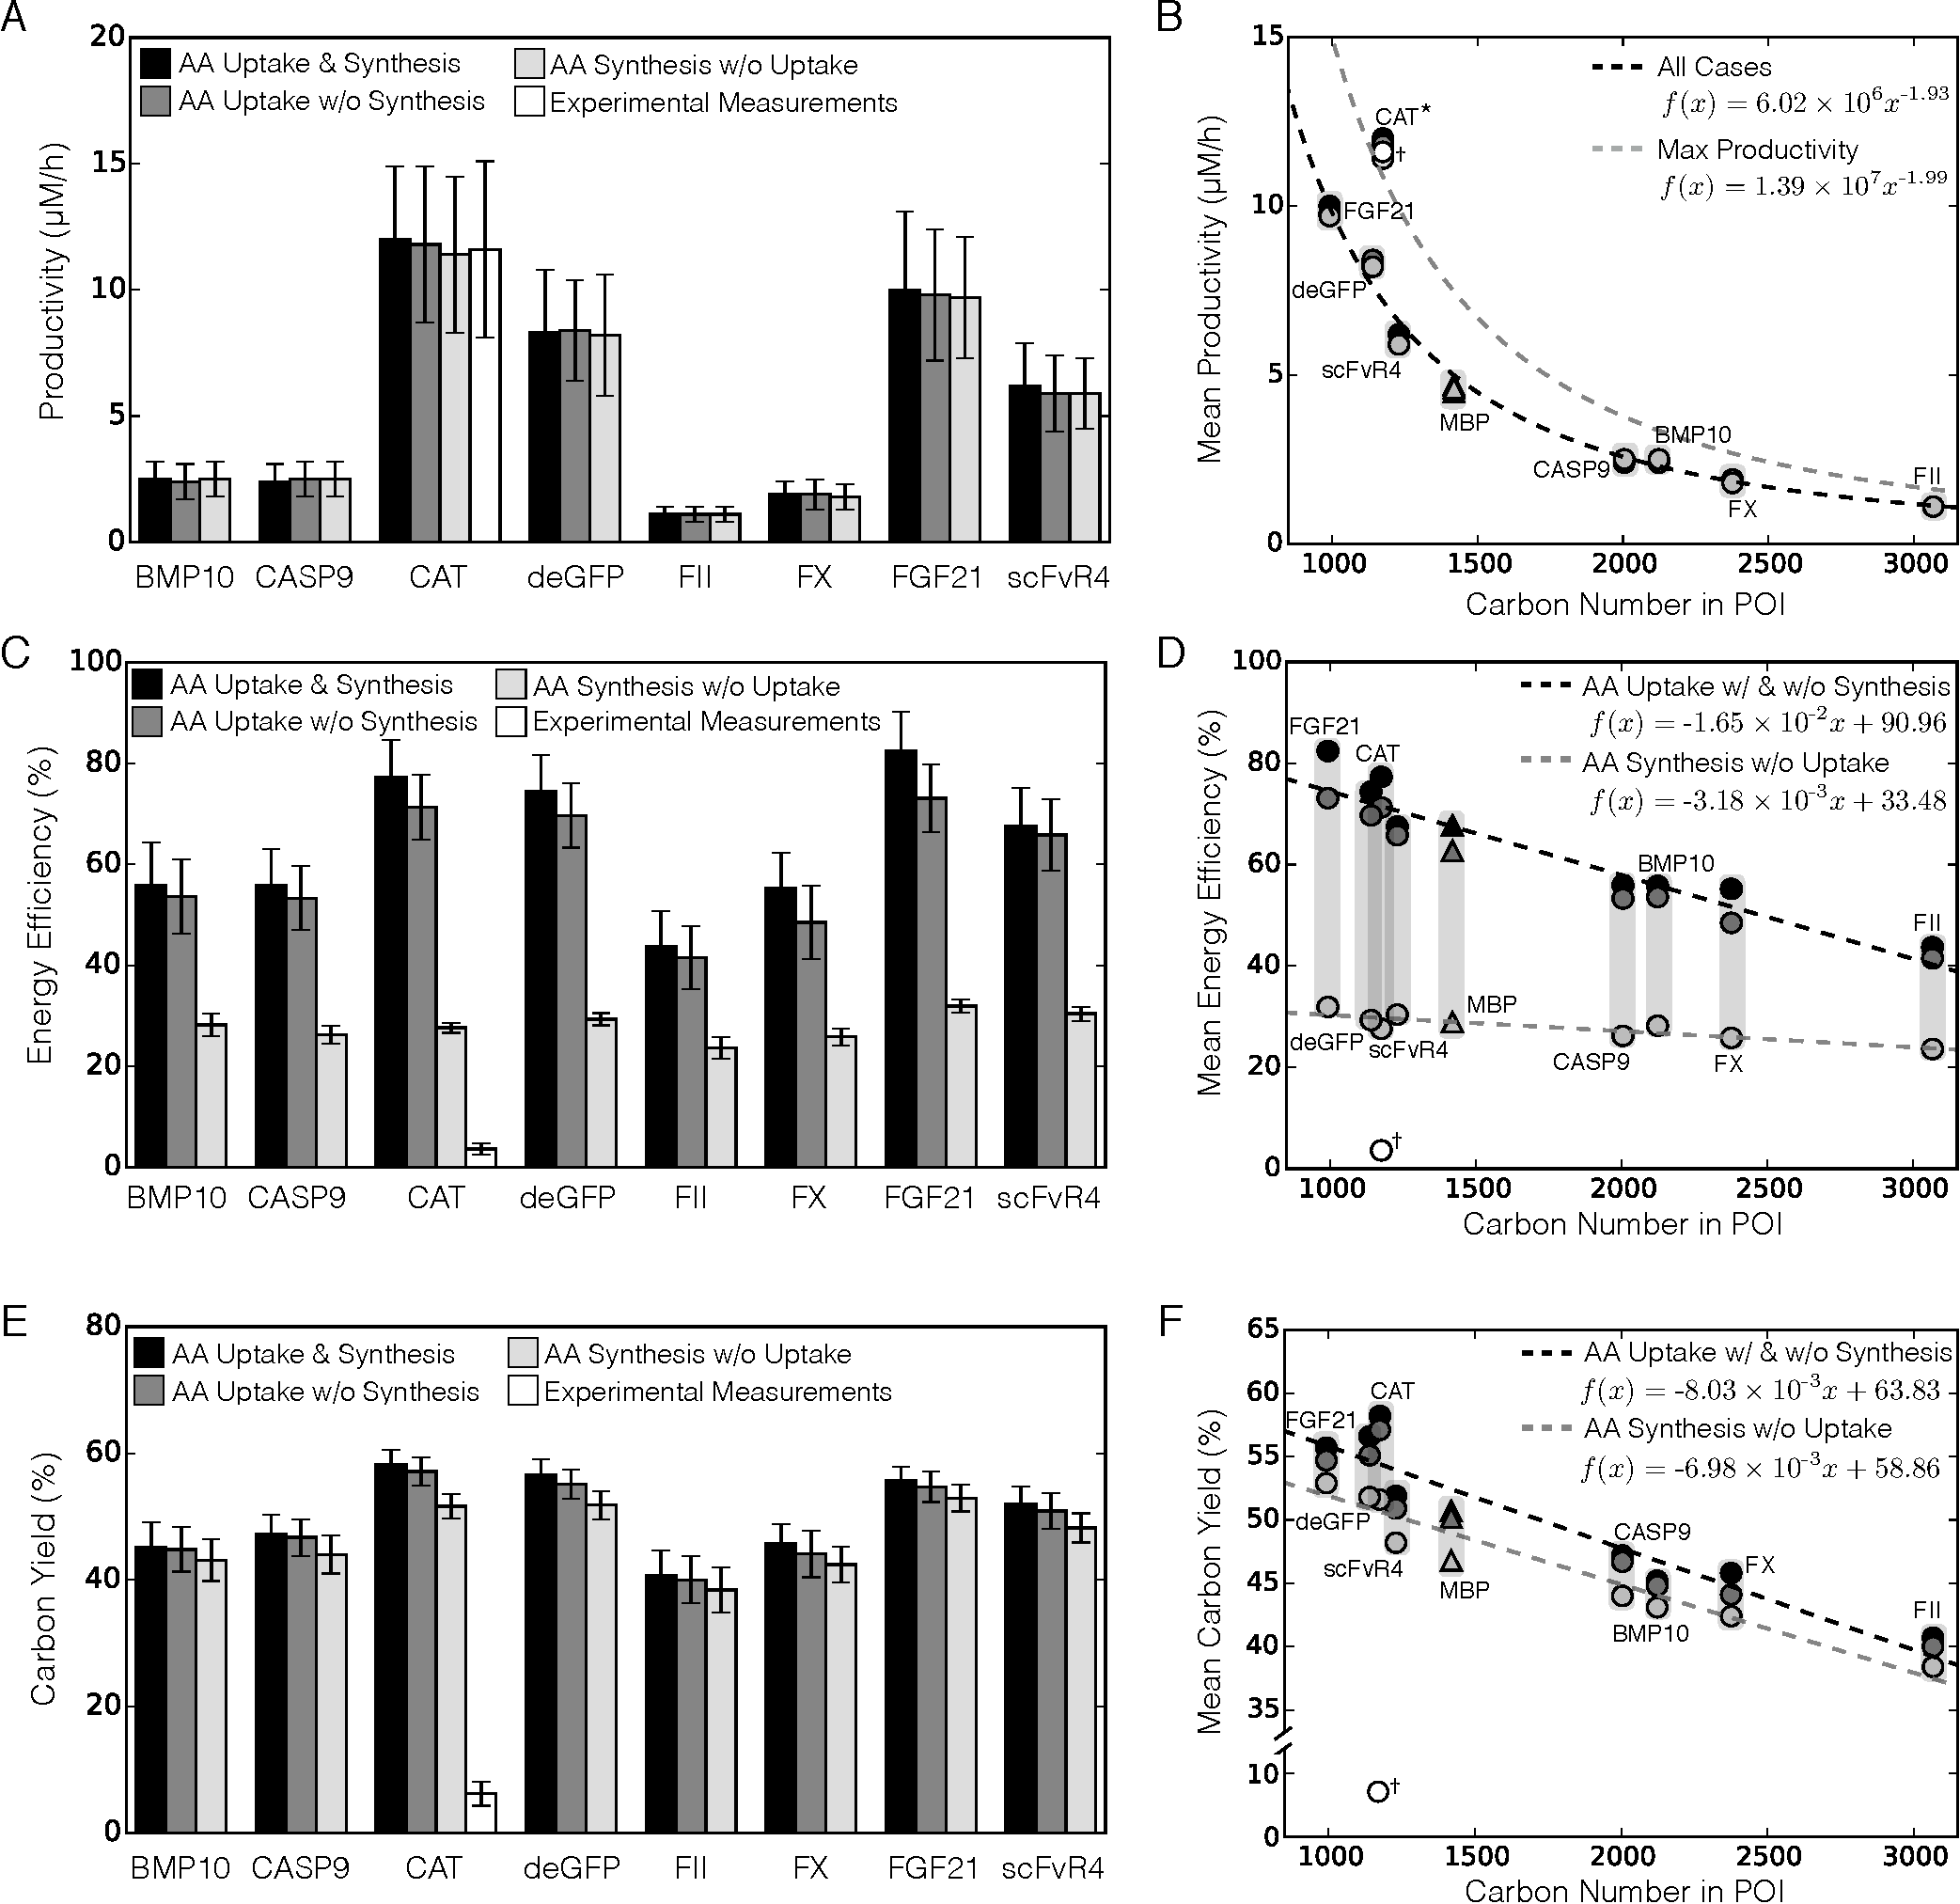
\includegraphics[width=1.00\textwidth]{./figs/Fig-2-Performance.pdf}
%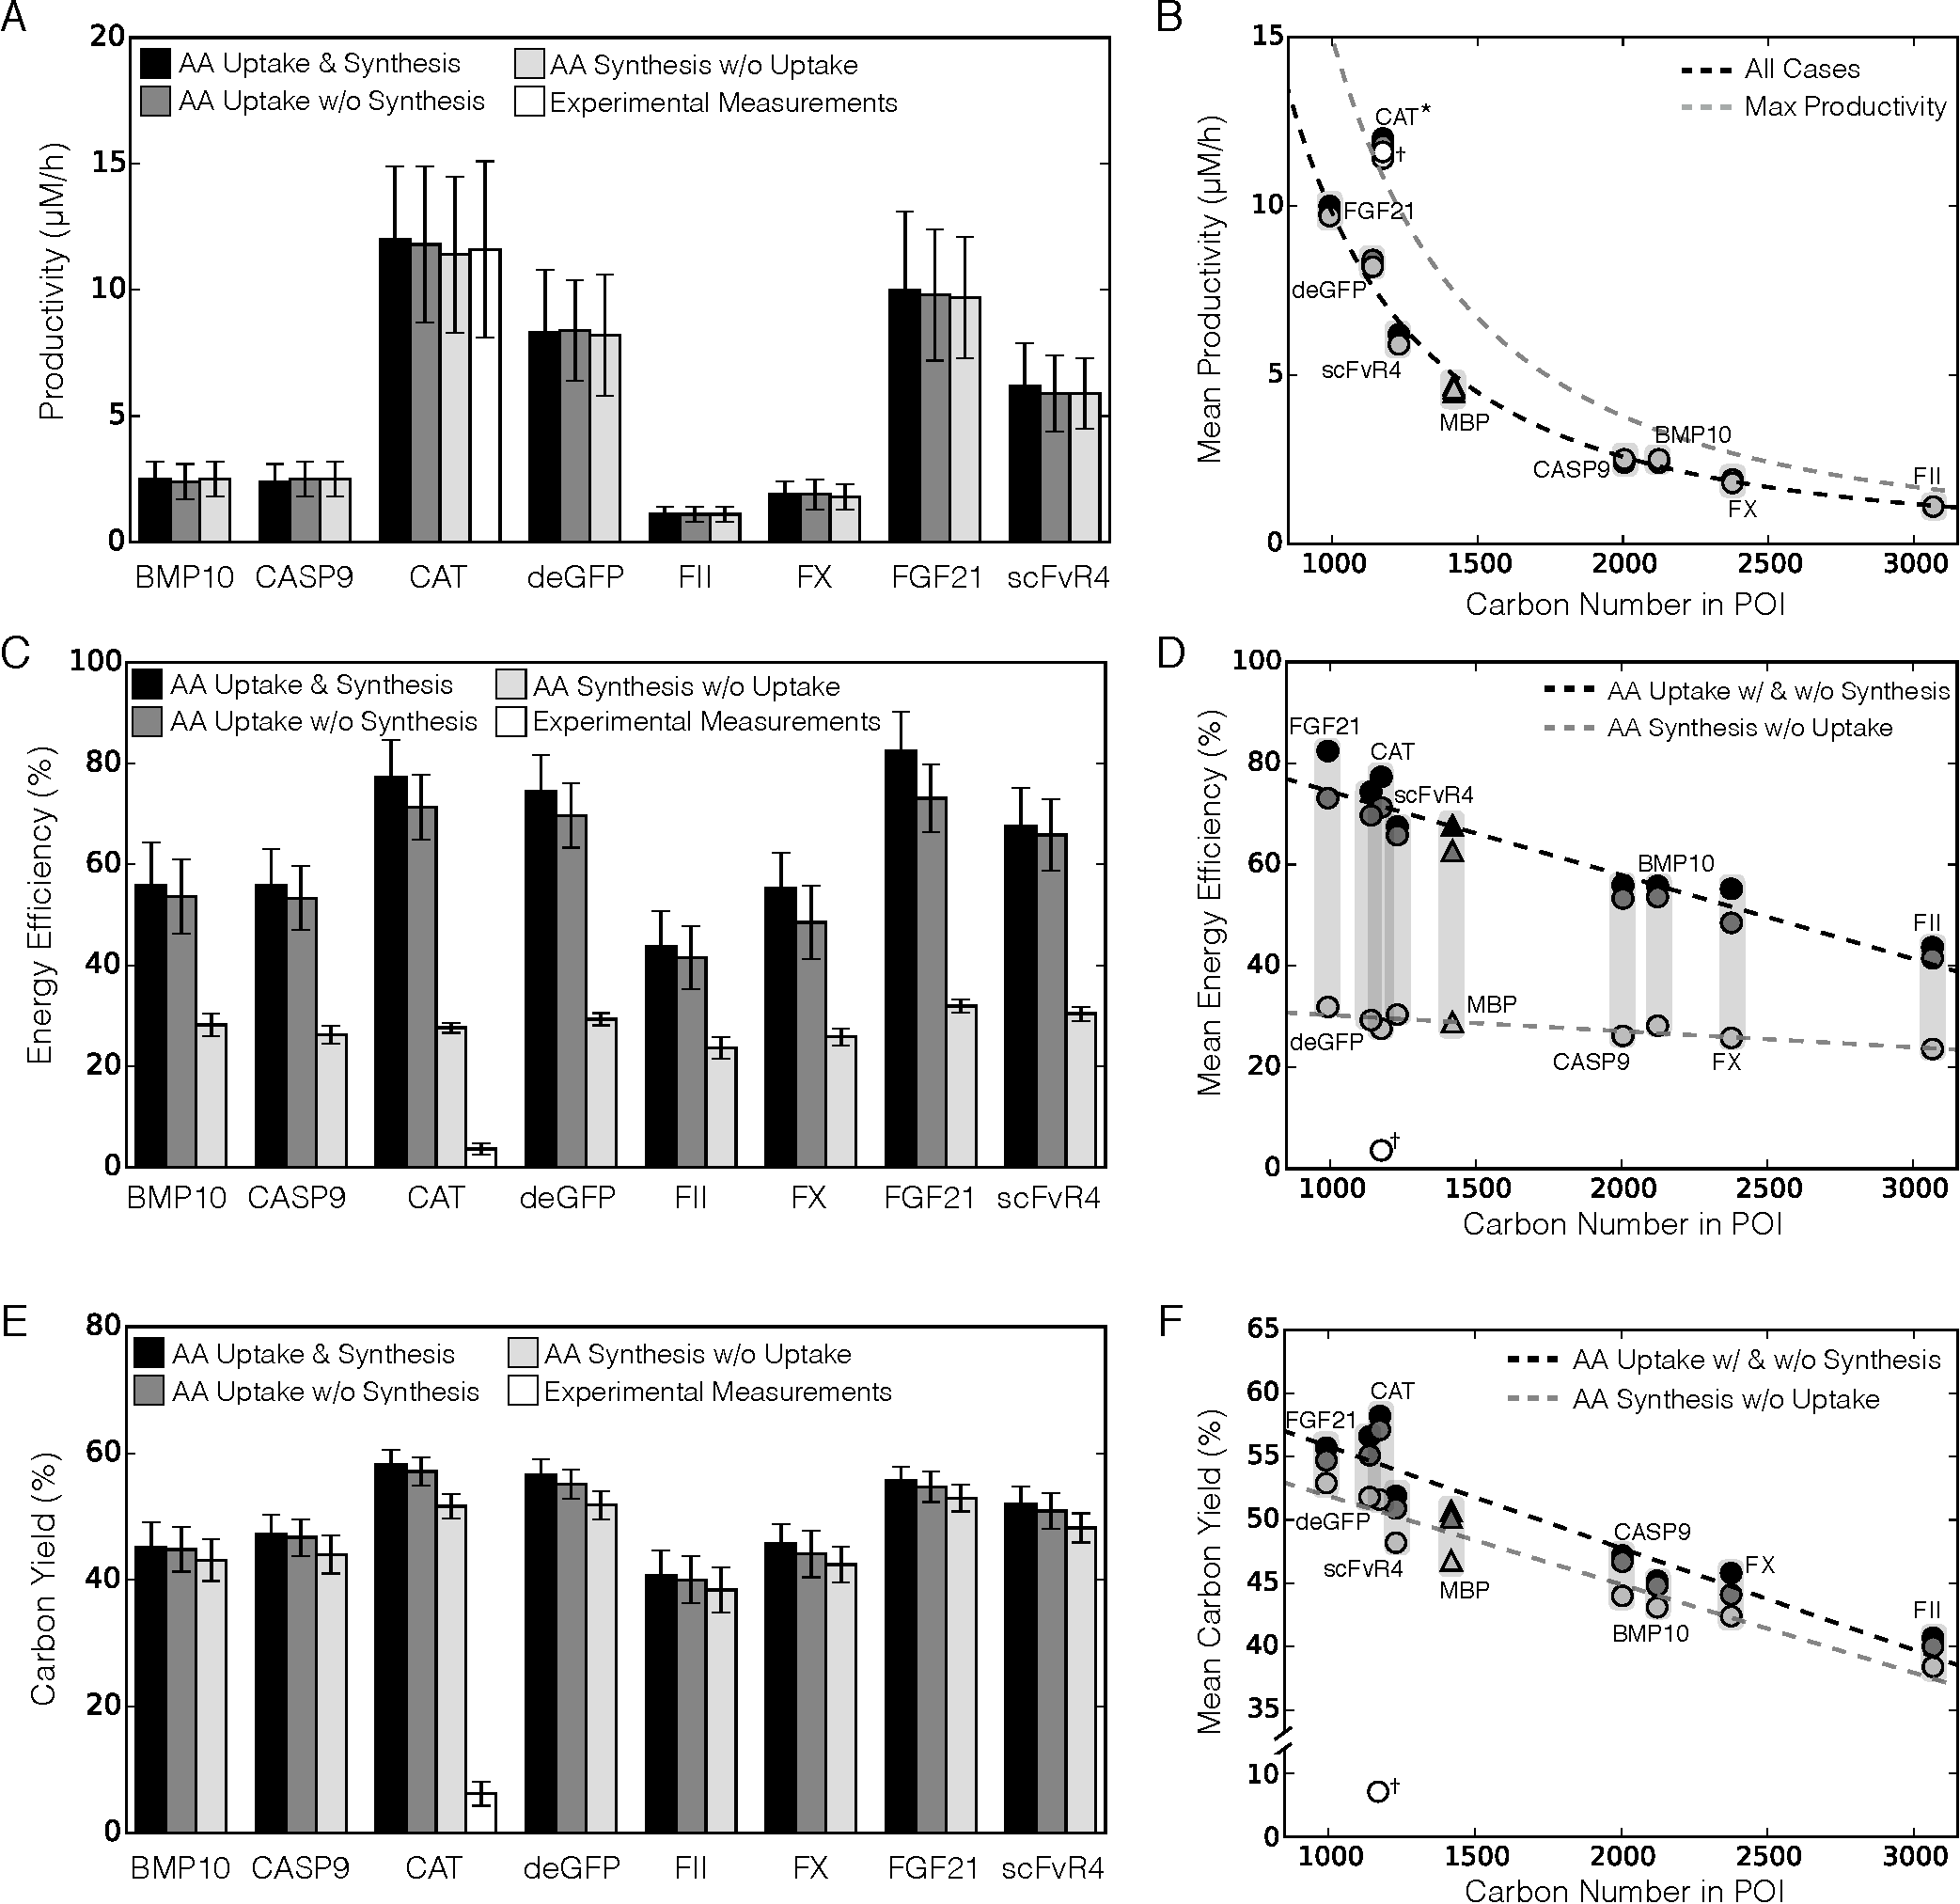
\includegraphics[width=1.00\textwidth]{./figs/Fig-2-Performance-Predicted.pdf}
\caption{CFPS performance of eight proteins for four cases. Amino acid uptake and synthesis (black), AA uptake without synthesis (dark grey), AA synthesis without uptake (light grey), and constrained by experimental measurements, for CAT only (white). A. Productivity. B. Mean productivity versus carbon number. Single trendline (black dotted line) calculated across all cases (R\textsuperscript{2} = 0.99) and maximum productivity trendline (grey dotted line; R\textsuperscript{2} = 0.99) .
C. Energy efficiency. D. Mean energy efficiency versus carbon number. Trendline for cases with amino acids (black dotted line; R\textsuperscript{2} = 0.91) and trendline for without amino acids (grey dotted line; R\textsuperscript{2} = 0.78).
E. Carbon yield. F. Mean carbon yield versus carbon number. Trendline for cases with amino acids (black dotted line; R\textsuperscript{2} = 0.95) and trendline for without amino acids (grey dotted line; R\textsuperscript{2} = 0.90).
Error bars: 95\% CI; asterisk: protein excluded from trendline; dagger: constrained by experimental measurements and excluded from trendline; triangles: first principle prediction and excluded from formulating trendline.}
\label{fig:Prof}
\end{figure}

\subsubsection{Productivity}
The theoretical maximum productivity for proteins expressed using a P70a promoter ($\mu$M/h) was inversely proportional to the carbon number ($C_{POI}$) and varied between 1 and 12 $\mu$M/h for the proteins sampled (Fig.~\ref{fig:Prof}A-B).
The theoretical maximum productivity was within a standard deviation with and without amino acid supplementation for each protein, but varied significantly between proteins.
Moreover, productivity was a non-linear function of protein length; for instance, BMP10 (424 aa) had a optimal productivity of approximately 2.5 $\mu$M/h whereas CAT (219 aa) had an optimal productivity of approximately 12 $\mu$M/h.
To examine the influence of protein length further, the mean optimal productivity was plotted against the carbon number of each protein (Fig.~\ref{fig:Prof}B).
The optimal productivity and protein length were related by the power-law relationship $\alpha\times(C_{POI})^{\beta}$, where $\alpha = 6.02\times 10^{6}$ $\mu$M/(h$\cdot$carbon number) and $\beta=-1.93$.
Interestingly, CAT did not obey the power-law relationship; the relatively high productivity of CAT was due to its T7 promoter.
The higher transcription rate of the T7 promoter led to a 34\% higher mRNA steady state level, resulting in a higher productivity.
Thus, we also calculated the theoretical productivity correlation given maximum promoter activity using all eight proteins which resulted with $\alpha = 1.39\times 10^{7}$ $\mu$M/(h$\cdot$carbon number) and $\beta=-1.99$.
However, CAT expressed under a P70a promoter followed the power-law correlation with a productivity of approximately 8.2 $\pm$ 2.2 $\mu$M/h (predicted to be 7.2 $\mu$M/h by the optimal productivity correlation).
Different promoters have been shown to have different strengths which have effected the productivity of proteins in CFPS \cite{Moon:2012ab,Garamella:2016aa}; this is consistent with our results for CAT productivity on a T7 and P70a promoter.
In addition, to evaluate the accuracy  of our productivity P70a model, we predicted the productivity of MBP to be 4.6 $\mu$M/h whereas the power-law relationship predicted a productivity of 5.0 $\mu$M/h.
This difference in prediction was less than 8\% error in estimating the productivity of an \emph{a~priori} protein in CFPS.
Taken together, the maximum optimal productivity of a cell-free reaction was found to be inversely proportional to protein size,
following a power-law relationship for proteins expressed under a P70a promoter.

% Taken together, a single trendline showed good agreement (R\textsuperscript{2} = 0.99) with estimating the expected productivity of a protein on a  in CFPS, given the size of the protein.
%The higher productivity of CAT compared to all other proteins was most likely due to the lower transcription requirement of cytidine triphosphate which allowed a higher flux for translation.
% further study on the nucleotide and amino acid requirements of each protein and its effect on CFPS performance should be investigated.


\subsubsection{Energy efficiency}
The energy efficiency of protein synthesis was linearly related to protein carbon number, both with and without amino acid supplementation (Fig.~\ref{fig:Prof}C-D).
However, the dependence of energy efficiency on carbon number was less pronounced in the absence of amino acid supplementation.
The relationship between the optimal energy efficiency and carbon number was linear; $m_{Y}\times(C_{POI})+b_{Y}$ where $m_{Y} =  -1.65\times10^{-2}$ energy efficiency (\%)/carbon number with supplementation,
and $m_{Y} = -3.18\times10^{-3}$ energy efficiency (\%)/carbon number without supplementation.
The y-intercept $b_{Y} = 90.96$ energy efficiency (\%) with supplementation, and $b_{Y} = 33.48$ energy efficiency (\%) without.
Proteins with a high carbon number had a lower energy efficiency since they have higher transcription and translation costs compared with smaller proteins.
However, this effect was less pronounced in the absence of supplementation, where the optimal energy efficiency was a weaker function of the protein carbon number.
MBP showed good agreement with the formulated relationship between energy efficiency and carbon number for each case.
The estimated MBP energy efficiency had a maximum error of 7.1\% for the case where amino acid biosynthesis reactions were blocked and an error of 0.2\% for both remaining cases.
The cases supplemented with amino acids had the same trendline whereas when amino acids were not available there was a significant drop in energy efficiency.
Interestingly, without supplemented amino acids each protein had a similar energy efficiency ranging between 24-32\% regardless of carbon number.
In this case, the glucose uptake relatively doubles (64\% increase for CAT) compared to cases supplemented with amino acids, meanwhile the productivity stays relatively the same for each protein (Fig.~\ref{fig:Prof}D).
Therefore the energy burden (i.e. higher glucose uptake) for synthesizing each amino acid and powering CFPS has kept the energy efficiency saturated at a relatively low level, regardless of the protein.
However, the experimentally constrained case of CAT production showed even a lower energy efficiency of 3.6 $\pm$ 1.1\% compared to the theoretical maximum of 77.3 $\pm$ 7.3\%.
This shows CFPS systems are not fully optimized and could be improved: first, the experimental measurements showed accumulation of certain amino acids; this carbon could potentially be diverted towards a protein of interest.
Second, the system had a high accumulation of metabolic byproducts, specifically organic acids, which was a result of inefficient energy utilization.

% With amino acid supplementation, there was a comparable energy efficiency, despite the network's ability to synthesis amino acids.
% For the case when amino acids were removed from the media, protein production resulted in a low energy efficiency; below 32\% depending on the protein.
% This was because glucose had to be utilized to synthesize the amino acids necessary for protein synthesis and meet the necessary energy demands of CFPS.
% %We next investigated the effect of protein carbon number on energy efficiency (Fig.~\ref{fig:Prof}D).
% The same inverse trend was observed as for productivity for the effect of protein carbon number on energy efficiency, except that it was linear
%
%
% %The proteins with the lowest carbon number had the highest energy efficiency and the higher carbon number proteins had a lower energy efficiency for when amino acids were available in the media (first two cases).
%This may be a potential area for improvement in CFPS to optimize for energy utilization.
% \begin{figure}[t!]
% \centering
% 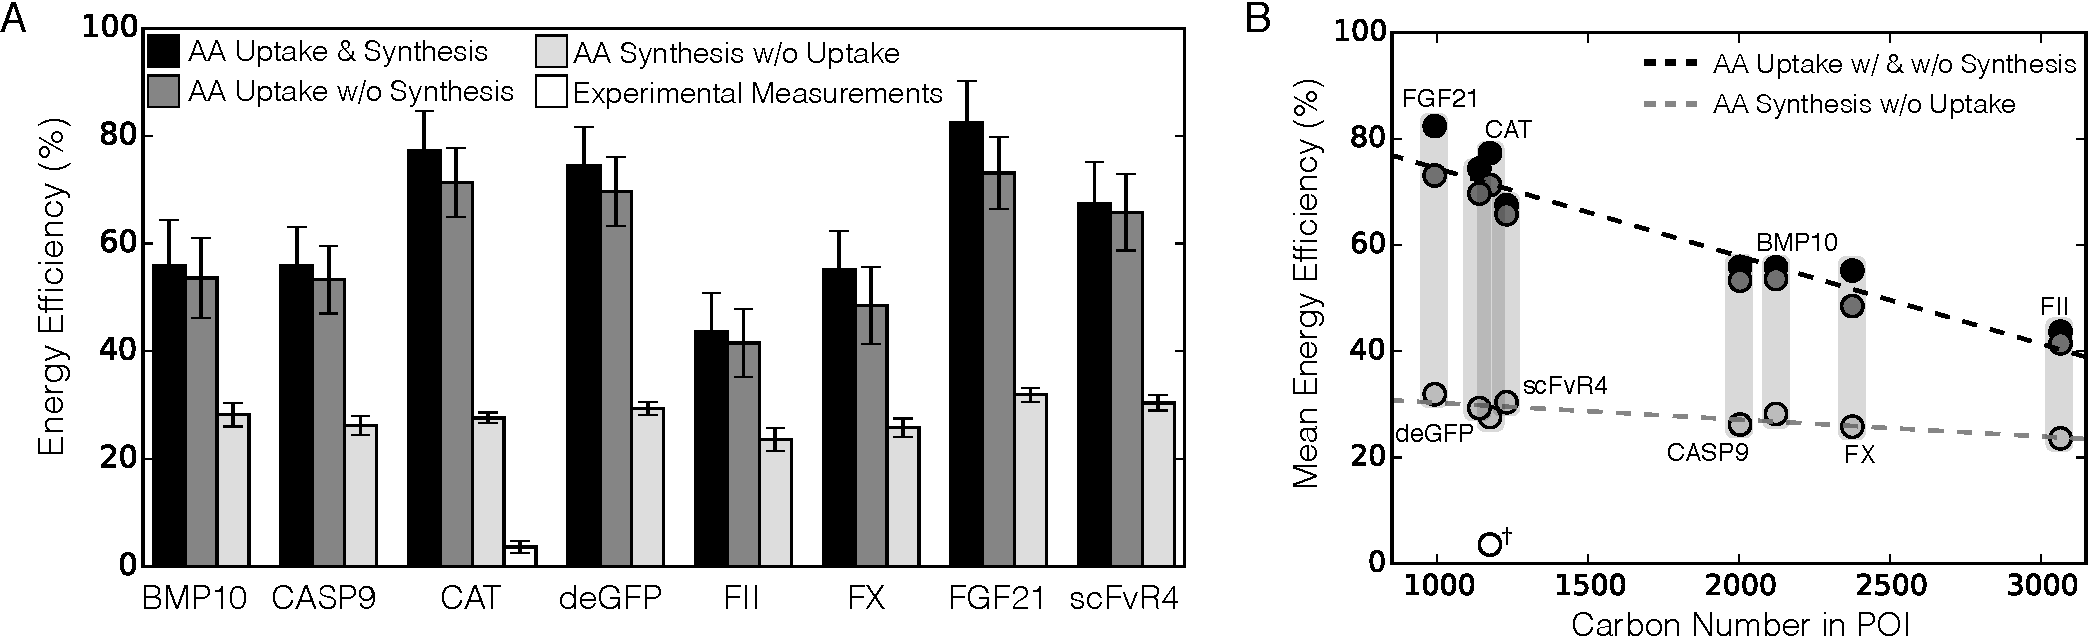
\includegraphics[width=1.00\textwidth]{./Figures/Energy.pdf}
% \caption{CFPS energy efficiency of eight proteins for four cases. Amino acid uptake and synthesis (black), AA uptake without synthesis (dark grey), AA synthesis without uptake (light grey), and constrained by experimental measurements, for CAT only (white). A. Energy efficiency (Error bars represent the 95\% CI of the ensemble). B. Mean energy efficiency versus the carbon number for each corresponding protein. Trendline of energy efficiency versus carbon number (black dotted line) for first two cases (y = -1.65$\cdot$10\textsuperscript{-2}x+90.95; R\textsuperscript{2} = 0.91) and trendline for AA synthesis without uptake (grey dotted line; y = -3.18$\cdot$10\textsuperscript{-3}x+33.48; R\textsuperscript{2} = 0.78). Dagger: constrained by experimental measurements and excluded from trendline.}
% \label{fig:Energy}
% \end{figure}

%To determine the carbon contribution from each substrate (glucose and amino acids) we examined the carbon flux going toward the production of deGFP for all three cases (Table \ref{tbl:yield_breakdown}).
%The cases supplemented with amino acids in the media showed the highest carbon yield.
%Finally, for the third case (without amino acids supplemented), the carbon yield was reduced to 51.1 $\pm$ 1.8\% for CAT, and the system used about twice the amount of glucose as in the first two cases.
%In this case, glucose was used to synthesize amino acids and provide the energy necessary to power transcription and translation; this trend was seen across all proteins.
% W, the system relied on a mixture of glucose and some amino acids for each protein with a carbon yield of 58.2 $\pm$ 2.3\% for CAT.
% Once amino acid synthesis reactions were blocked in the network (second case), the carbon yield dropped to 57.1 $\pm$ 2.2\% for CAT.

\subsubsection{Carbon Yield}
The theoretical maximum carbon yield was inversely proportional to protein length and varied between 40\% and 57\% for the proteins sampled (Fig.~\ref{fig:Prof}E-F).
The relationship between the optimal carbon yield and carbon number was linear; $m_{Y}\times(C_{POI})+b_{Y}$ where $m_{Y} =  -8.03\times10^{-3}$ carbon yield (\%)/carbon number with supplementation, and $m_{Y} = -6.98\times10^{-3}$ carbon yield (\%)/carbon number  without. The y-intercept $b_{Y} = 63.83$ carbon yield (\%) with supplementation, and $b_{Y} = 58.86$ carbon yield (\%) without.
The linear carbon yield models showed good predictability for estimating the optimal carbon yield for a range of carbon numbers ($R^{2} = 0.95$ with amino acids
and $R^{2} = 0.90$ without supplementation), irrespective of the promoter used to control protein expression.
MBP also showed good agreement for its predicted carbon yield with the formulated relationship with an error of 3.2-4.2\% with amino acid supplementation and 4.4\% error without supplementation.
The effective yield models were approximately parallel, with a drop in carbon yield of approximately 7\% without amino acids.
%In this case, there is a higher uptake of glucose and an increase in CO\textsubscript{2} production by 37-40\% and acetate production by 4-14\%.
In this case, there was a higher uptake of glucose and an increase of CO\textsubscript{2} production in the carbon yield by 7\%.
Only the necessary amount of amino acids were used for the production of the protein of interest; thus, it may be hypothesized that all the glucose was used to power CFPS and did not contribute to the carbon yield.
The carbon yield without the glucose contribution would be 100\%.
However, in the experimentally constrained case, CAT was produced with a carbon yield of 6.2\% compared to the theoretical maximum of 58\%.
This decrease in carbon yield suggests inefficiencies in CFPS that can potentially be improved.
Constraint based calculations assume a metabolic pseudo steady state; thus, intermediate metabolites cannot accumulate within the cell-free extract.
In addition, the flux balance analysis calculation is solved by maximizing the flux through the protein production reaction.
Therefore, carbon flux will travel through the network to optimize the maximum flux through the protein synthesis reaction.
In examining the experimental dataset, there is a high accumulation of organic acids, especially acetate, pyruvate and lactate.
The experimental performance could be improved by diverting this carbon toward the protein of interest by knockouts during the cell-free extract preparation.

% \begin{figure}[t!]
% \centering
% 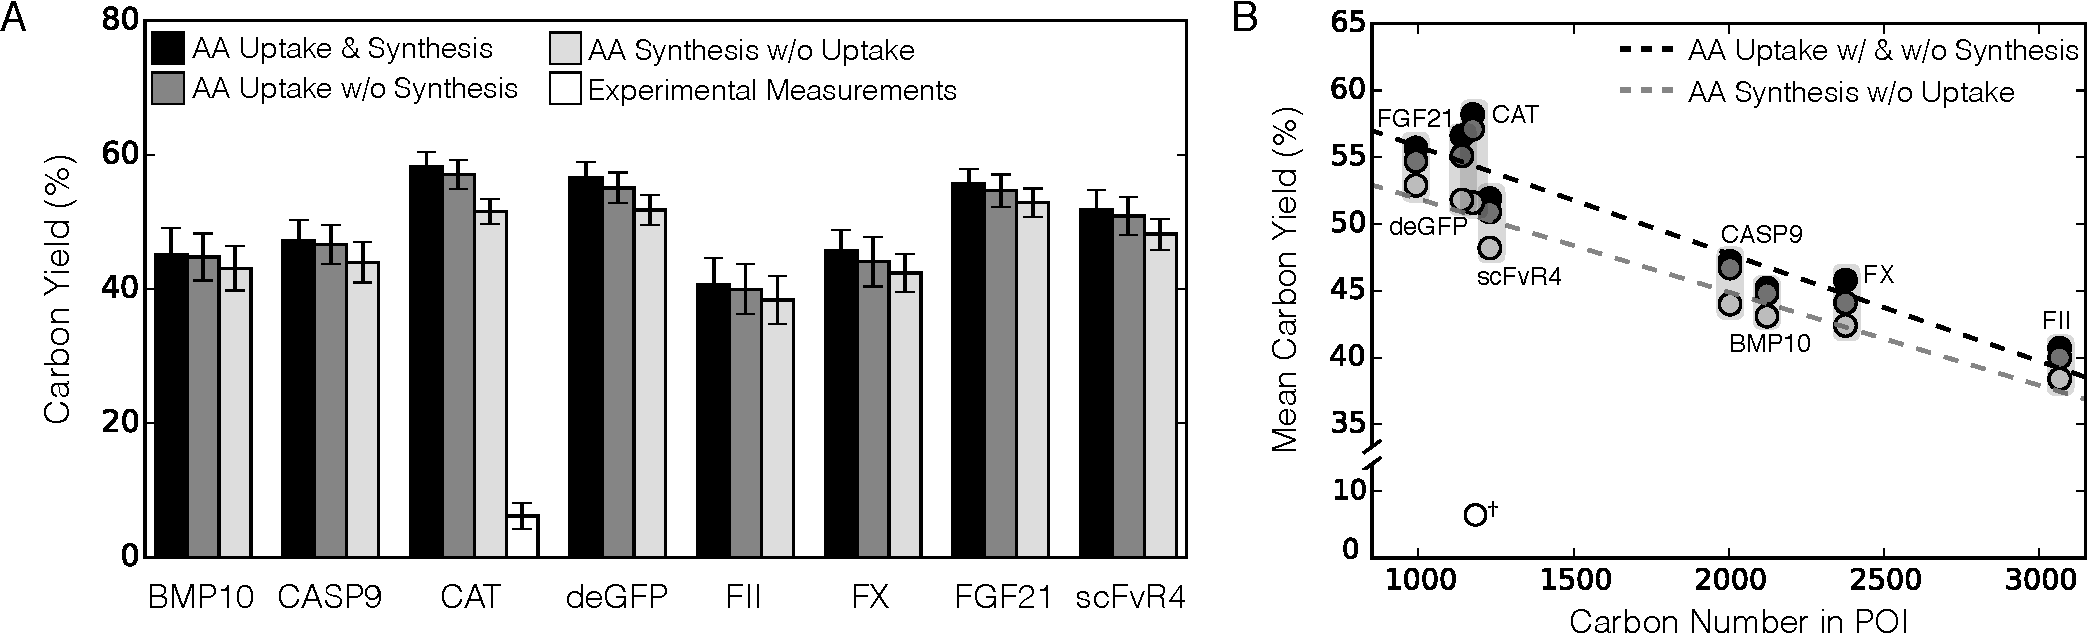
\includegraphics[width=1.00\textwidth]{./Figures/Yield.pdf}
% \caption{CFPS carbon yield of eight proteins for four cases. Amino acid uptake and synthesis (black), AA uptake without synthesis (dark grey), AA synthesis without uptake (light grey), and constrained by experimental measurements, for CAT only (white). A. Energy efficiency across the ensemble (error bars represent the 95\% CI). B. Mean energy efficiency versus the carbon number for each corresponding protein. Trendline of energy efficiency versus carbon number (black dotted line) for first two cases (y = -8.03$\cdot$10\textsuperscript{-3}x+63.83; R\textsuperscript{2} = 0.95) and trendline for AA synthesis without uptake (grey dotted line; y = -6.98$\cdot$10\textsuperscript{-3}x+58.86; R\textsuperscript{2} = 0.90). Dagger: constrained by experimental measurements and excluded from trendline.}
% \label{fig:Yield}
% \end{figure}
%Next we investigated the effect of the carbon number of each protein on the carbon yield (Fig.~\ref{fig:Yield}B).
%The proteins with the lowest carbon number had the highest yield and the higher carbon number proteins had a lower carbon yield within each case.
% A single trendline was formulated for the cases where amino acids were supplied in the media since they had similar performance, while another trendline was formulated for when amino acids were not available (Fig.~\ref{fig:Prof}F).

% Thus, we examined the parameters that had the most significant effect on cell-free productivity, energy efficiency, and carbon yield in order to optimize CFPS performance.

\subsection{Global sensitivity analysis}
To better understand the effect of substrate utilization and the transcription/translation parameters on CFPS performance, we performed global sensitivity analysis on the productivity, energy efficiency and carbon yield for the CAT protein (Fig.~\ref{fig:SI}).
Surprisingly, RNAP and ribosome abundance had only a modest effect;
the translation elongation rate had the largest effect on protein productivity.
On the other hand, oxygen followed by substrate consumption had the largest influence on the energy efficiency and carbon yield, respectively.
The significance of transcription/translation parameters was robust to amino acid supplementation, with the translation rate being the most sensitive across all cases (Fig.~\ref{fig:SI}A).
This suggested that the translation elongation rate, and not transcriptional parameters, controlled productivity.
Underwood and coworkers showed that an increase in ribosome levels did not significantly increase protein yields or rates; however, adding elongation factors increased protein synthesis rates by 33\% and yields by 23\% at 30 minutes \cite{2005_underwood_biotech}.
In addition, Li et al. increased the productivity of firefly luciferase production in PURE CFPS by 5-fold by adjusting factors that affect transcription and translation such as elongation factors, ribosome recycling factor, release factors, chaperones, BSA, and tRNAs \cite{2014_li_PlosOne}.
In examining substrate utilization, glucose consumption was not important for productivity in the presence of amino acid supplementation.
However, its importance increased significantly when amino acids were not available.
On the other hand, amino acid consumption was only sensitive when amino acids synthesis reactions were blocked, as it was the only source of amino acids for CAT synthesis.
\begin{figure}[t!]
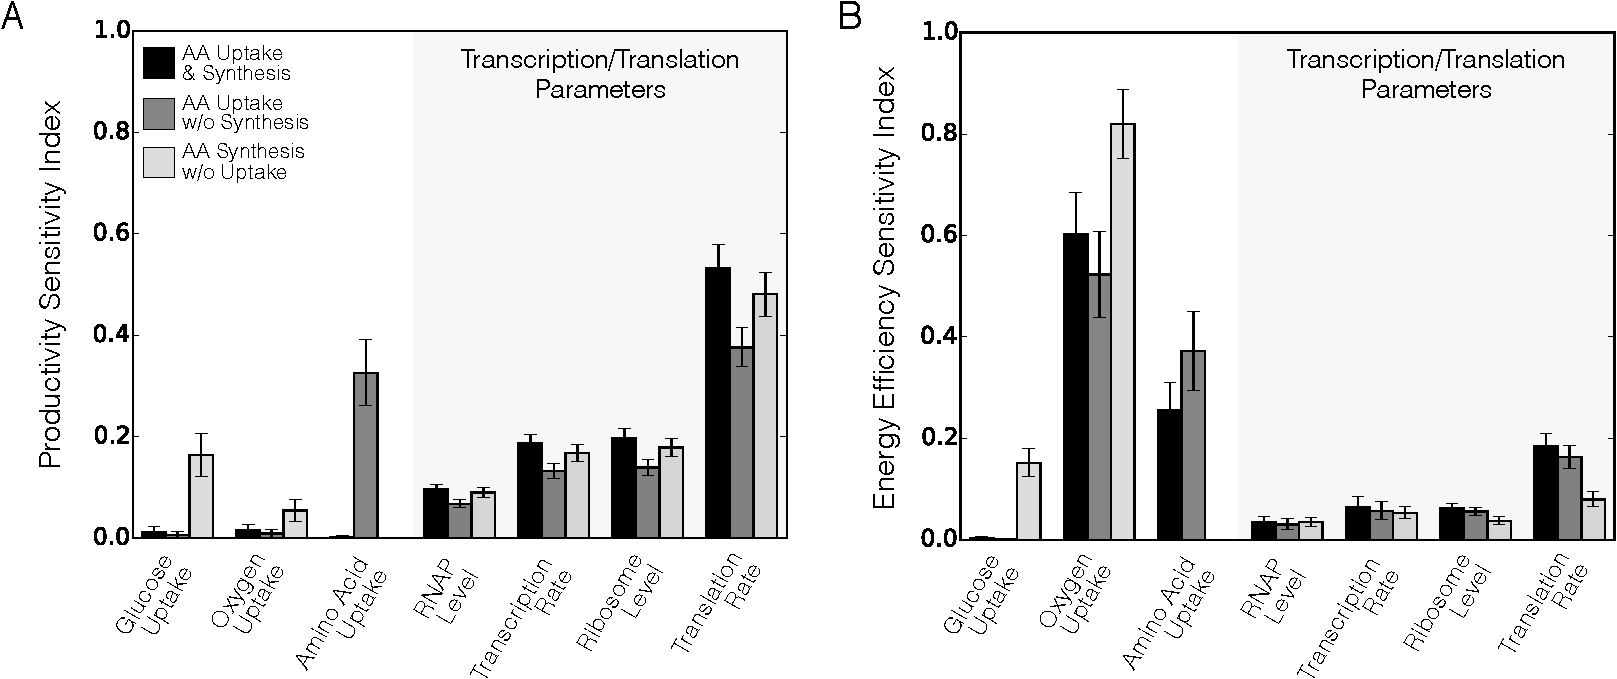
\includegraphics[width=1.00\textwidth]{./figs/Fig-3-Sensitivity-Analysis.pdf}
\caption{Total order sensitivity of deGFP productivity (A) and energy efficiency (B) to specific uptake rates and transcription/translation parameters for three cases: amino acid uptake and synthesis (black), amino acid uptake without synthesis (dark grey), and amino acid synthesis without uptake (light gray). Error bars represent a 95\% CI on the sensitivity index.}
\label{fig:SI}
\end{figure}

% The transcription/translation parameters had the same trend as for productivity, where the translation rate was the most sensitive compared to the other transcription/translation parameters and showed significance across all cases.

The oxygen consumption rate was the most important factor controlling the energy efficiency of cell-free protein synthesis (Fig.~\ref{fig:SI}B).
In addition to the oxygen consumption, amino acid utilization was also sensitive.
On the other hand, glucose consumption was only sensitive in the absence of amino acid supplementation,
since glucose acted as the sole source of carbon and energy for protein synthesis.
In the model, we assumed that ATP could be produced by both substrate level and oxidative phosphorylation.
Jewett and coworkers reported that oxidative phosphorylation still operated in cell-free systems, and that the protein
yield decreased from 1.5-fold to 4-fold when oxidative phosphorylation reactions were inhibited in pyruvate-powered CFPS \cite{Jewett:2008aa}.
However, it is unknown how active oxidative phosphorylation is for a glucose powered cell-free system.
Moreover, the connection between oxidative phosphorylation activity and other performance metrics, such as the carbon yield, is also unclear.

To investigate the connection between carbon yield and oxidative phosphorylation further,
we calculated the CAT carbon yield as a function of the oxidative phosphorylation flux (Fig.~\ref{fig:oxphos_yield}).
Oxidative phosphorylation had a strong effect on the carbon yield, both with and without amino acid supplementation.
In the presence of amino acid supplementation, the carbon yield ranged from 20\% to approximately 60\%,
depending upon the oxidative phosphorylation flux.
However, without amino acid supplementation, the carbon yield dropped to approximately 10\%, and reached a maximum of 50\%.
In the absence of supplementation, a lower carbon yield was expected for the same oxidative phosphorylation flux, as glucose was utilized for both energy generation and amino acid biosynthesis.
In all cases, whenever the carbon yield was below its theoretical maximum, there was an accumulation of both acetate and lactate.
The experimental dataset also exhibited a mixture of acetate and lactate accumulation during CAT synthesis, which suggested the CFPS reaction was not
operating with optimal oxidative phosphorylation activity.
Oxidative phosphorylation is a membrane associated process, however CFPS has no cell membrane.
Jewett et al. hypothesized that membrane vesicles present in the CFPS reaction carry out oxidative phosphorylation \cite{Jewett:2008aa}.
In addition, they were able to enhance the production yields of CAT by 33\% when the reaction was augmented with 10mM phosphate.
However, it is unclear why the additional phosphate increased the CAT yield, but Jewett et al. believe it either enhances oxidative phosphorylation activity or inhibits phosphatase reactions.
Taken together, the number, size, protein loading and lifetime of these vesicles remains an open area of study.
Thus, we expect CFPS will have suboptimal oxidative phosphorylation capacity and remains an important area to optimize for improved CFPS performance.

\begin{figure}[t!]
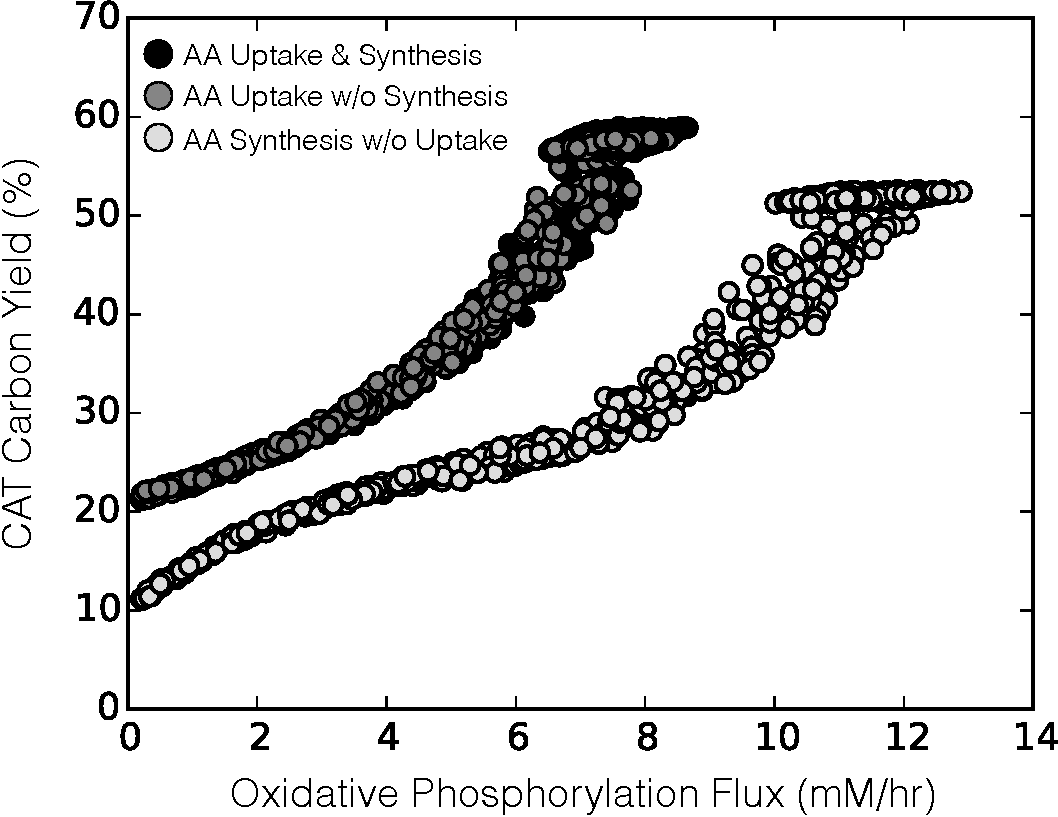
\includegraphics[width=0.7\textwidth]{./figs/Fig-4-OxyPhox-versus-Carbon-Yield.pdf}
\caption{The deGFP carbon yield versus oxidative phosphorylation flux, across an ensemble of 1000 flux balance solutions, for amino acid uptake and synthesis (black), amino acid uptake without synthesis (dark grey), and amino acid synthesis without uptake (light gray).}
\label{fig:oxphos_yield}
\end{figure}

\subsection{Optimal Metabolic Flux Distribution}
Amino acid supplementation altered the optimal metabolic flux distribution predicted for CAT production (Fig.~\ref{fig:flux}).
To investigate the influence of amino acid supplementation, we compared the simulated metabolic flux distributions for CAT production with and without external amino acids.
\begin{figure}[t!]
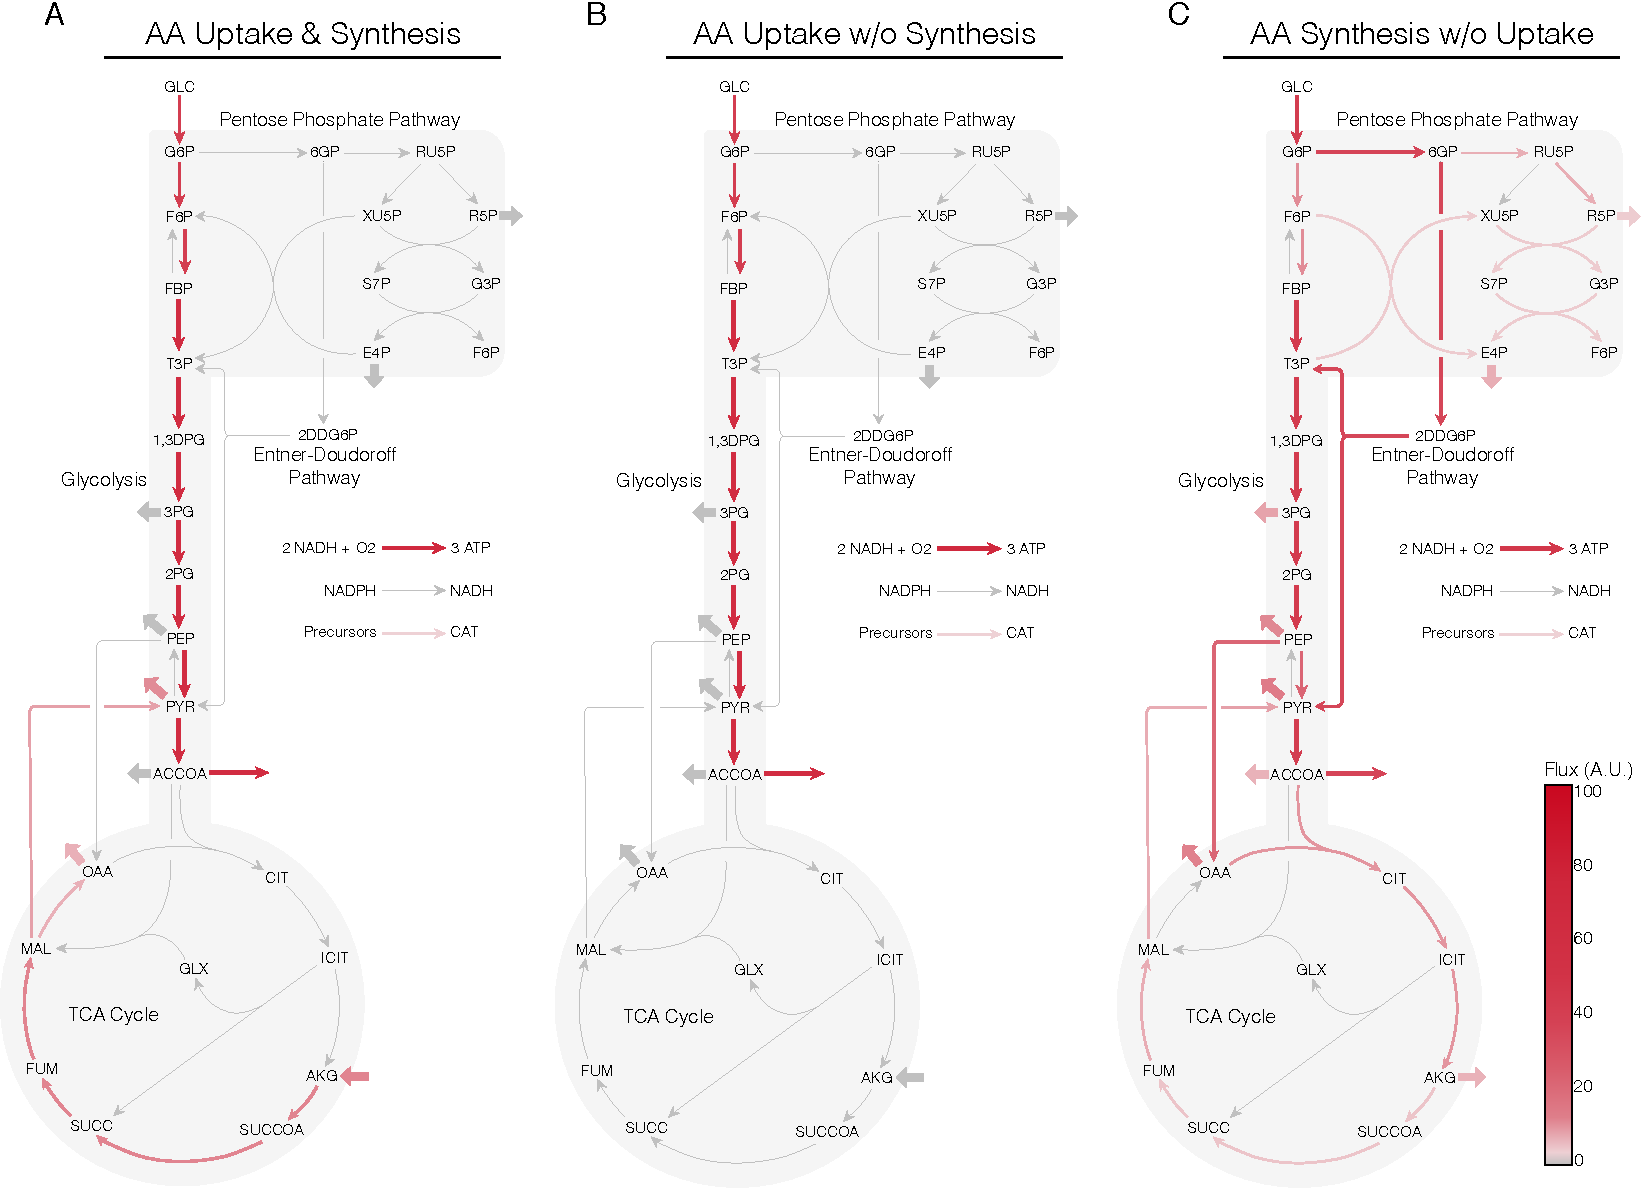
\includegraphics[width=1.00\textwidth]{./figs/Fig-5-FluxDistribition-Optimal.pdf}
\caption{Flux profile for glycolysis, pentose phosphate pathway, Entner-Doudoroff pathway, TCA cycle, and oxidative phosphorylation, for three different cases: (A) amino acid uptake and synthesis, (B) amino acid uptake without synthesis, and (C) amino acid synthesis without uptake. Mean flux across the ensemble, normalized to glucose uptake flux. Thick arrows indicate flux to or from amino acids.}
\label{fig:flux}
\end{figure}
In the presence of amino acid supplementation, and \textit{de~novo} amino acid synthesis, there was an incomplete TCA cycle, where a combination
of glucose and amino acids powered protein expression (Fig.~\ref{fig:flux}A).
Glucose was consumed to produce acetyl-coenzyme A, and associated by-products,
while glutamate was converted to alpha-ketoglutarate which traveled to oxaloacetic acid and pyruvate for additional amino acid biosynthesis.
On the other hand, in the presence of amino acid supplementation, but without \textit{de~novo} amino acid biosynthesis, there was no TCA cycle flux.
In this case, ATP was produced by a combination of substrate level and oxidative phosphorylation, where
ubiquinone was regenerated via \textit{nuo} activity, without relying on succinate dehydrogenase in the TCA cycle (Fig.~\ref{fig:flux}B).
These first two cases where amino acids were available had similar performance, and their respective metabolic flux distributions had a 99\% correlation for all proteins.
In the absence of amino acid supplementation (where all amino acids were synthesized \textit{de~novo} from glucose),
the energy efficiency and carbon yield decreased; in this case the TCA cycle was largely complete and there was diversion of metabolic flux into the Entner-Doudoroff pathway to produce NADPH (Fig.~\ref{fig:flux}C).
However, each of these three cases represent the theoretical optimum under different conditions; in order to more accurately describe system performance, we constrained the feasible solution space with experimental measurements.


% to both cases where amino acids were avaialbe.
% This drop in performance is due to the burden of synthesizing amino acids, which require NADPH.
% This leads to the relatively high flux in the first step of the pentose phosphate pathway to generate NADPH, thus, less NADH is available for oxidative phosphorylation.
% The performance metrics and sensitivity analysis suggest that efficient energy generation via oxygen uptake is essential to higher energy efficiency and carbon yields.
% %Thus, removing anaerobic enzymes during the cell-free extract preparation could potentially improve CFPS performance and protein yield.

The case constrained by experimental measurements (Fig. \ref{fig:flux_exp}) had the highest correlation of 0.66 with the flux distribution from the case supplied with no amino acids and a correlation of 0.52 with the cases supplied with amino acids.
Thus there are some differences in the flux distribution compared to the optimum solutions which may provide some insight to improve CFPS performance.
Metabolic fluxes were constrained by experimental measurements (available in Supporting Information) where available for the first hour
which constrained the feasible solution space.
The central carbon organic acids showed good agreement with the data with a coefficient of determination of R\textsuperscript{2}=0.92 (Fig.~\ref{fig:flux_exp}B).
Only certain amino acid synthesis reactions were blocked, since during the growth of \emph{E.~coli} not all amino acids were supplied (see Materials and Methods).
During the cell-free reaction all amino acids were supplied, however glucose still traveled through all the major pathways, and the same metabolic precursors were still utilized for amino acid biosynthesis.
In this case, it is unclear which substrate (glucose or amino acids) is used to power CFPS and may in fact be a combination of both.
The optimum solutions only produced the required amount of amino acids necessary, however in examining the measurements there is an accumulation of alanine and glutamine which may explain some of the differences in the correlations of the flux distributions.
Accumulation of pyruvate, lactate, acetate, and other organic acids can be seen (Fig.~\ref{fig:flux_exp}B) and is an inefficiency of carbon utilization.
\begin{figure}[t!]
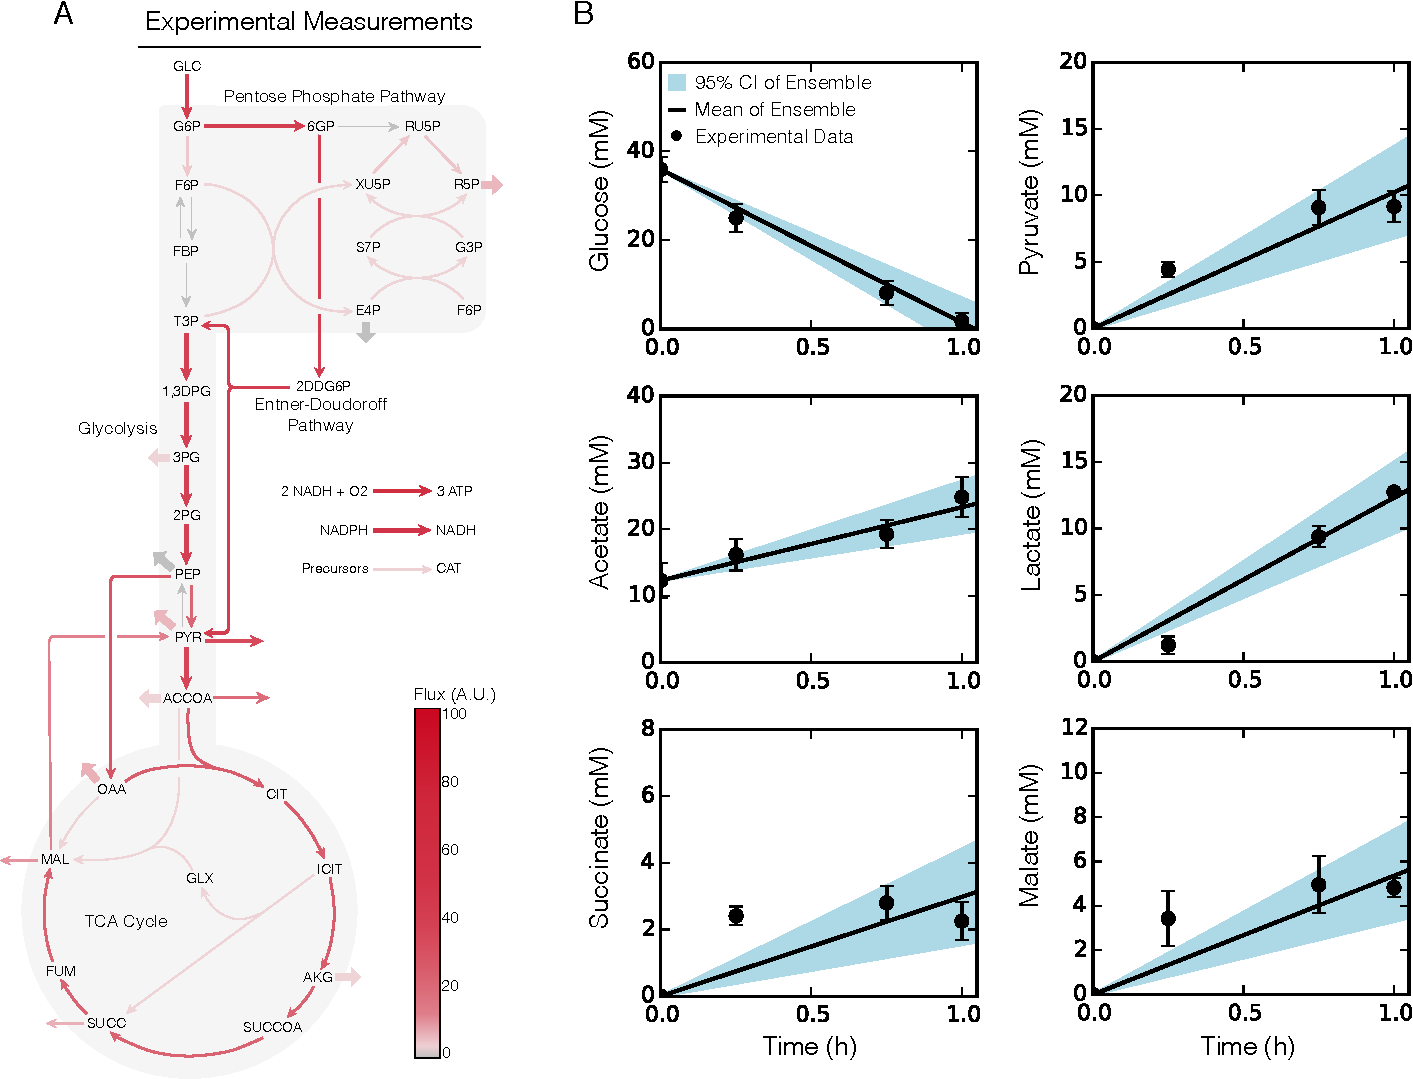
\includegraphics[width=1.00\textwidth]{./figs/Fig-6-FluxDistribition-Experimental.pdf}
\caption{Constraint based simulation of CAT production for an experimentally constrained case. (A) Flux profile for glycolysis, pentose phosphate pathway, Entner-Doudoroff pathway, TCA cycle, and oxidative phosphorylation.  Mean flux across the ensemble, normalized to glucose uptake flux. Thick arrows indicate flux to or from amino acids. (B) Central carbon metabolite measurements versus simulations over a one hour time course.}
\label{fig:flux_exp}
\end{figure}


\subsubsection{Potential Alternative Metabolic Optima}
Constraint based approaches can be used to compute alternative optimal solutions.
These solutions have the same objective value, e.g., productivity, but different underlying metabolic flux distributions.
Several techniques have been developed to estimate alternative optima, e.g., flux variability analysis \cite{Mahadevan2003264,Schuetz119} or mixed-integer approaches \cite{LEE2000711}.
In this study, we used reaction group flux variability analysis to estimate potential alternative optimal solutions for CAT production constrained by experimental measurements (Fig.~\ref{fig:norm}).
There were crucial pathways required for CAT production; for example, removal of the glycolysis/gluconoeogenesis or oxidative phosphorylation pathways resulted in no CAT production.
Likewise, there were also group knockouts that had no effect on productivity or the metabolic flux distribution, such as removal of isoleucine, leucine, and valine biosynthesis combined with histidine biosynthesis.
Globally, the constraint based simulation reached the same optimal CAT productivity for 40\% of the pairwise group knockouts, but had a different flux distribution when compared to the absence of knockouts.
For example, one of the features of the predicted optimal metabolic flux distribution was a high flux through the Entner-Douodoroff (ED) pathway.
Removal of the ED pathway had no effect on the CAT productivity compared to the absence of knockouts (Fig.~\ref{fig:norm}A).
Pairwise knockouts of the ED pathway and other subgroups (i.e. pentose phosphate pathway, cofactors, folate metabolism, etc.) also resulted in the same optimal CAT productivity.
However, there was a difference in the flux distribution with these knockouts (Fig.~\ref{fig:norm}B); thus, alternative optimal metabolic flux distributions exist for CAT production, despite experimental constraints.
In addition, knockouts of amino acid biosynthesis reactions had no effect on the productivity with the exception of ALA, ASP, ASN and GLU, GLN biosynthesis reactions, since amino acids were supplemented in the media.
ssFBA rerouted the metabolic flux to have the same productivity but an alterantive flux distribution (alternative optima), as can be seen for a pairwise knockout of GLY, SER biosynthesis with HIS biosynthesis (Fig.~\ref{fig:norm}B).
Ultimately, to determine the metabolic flux distribution occurring in CFPS, we need to add additional constraints to the flux estimation calculation.
For example, thermodynamic feasibility constraints may result in a better depiction of the flux distribution \cite{Henry:2007,Hamilton:2013},
and $^{13}$C labeling in CFPS could provide significant insight.
However, while $^{13}$C labeling techniques are well established for \emph{in~vivo} processes \cite{Zamboni:2009},
application of these techniques to CFPS remains an active area of research.
\begin{figure}[t!]
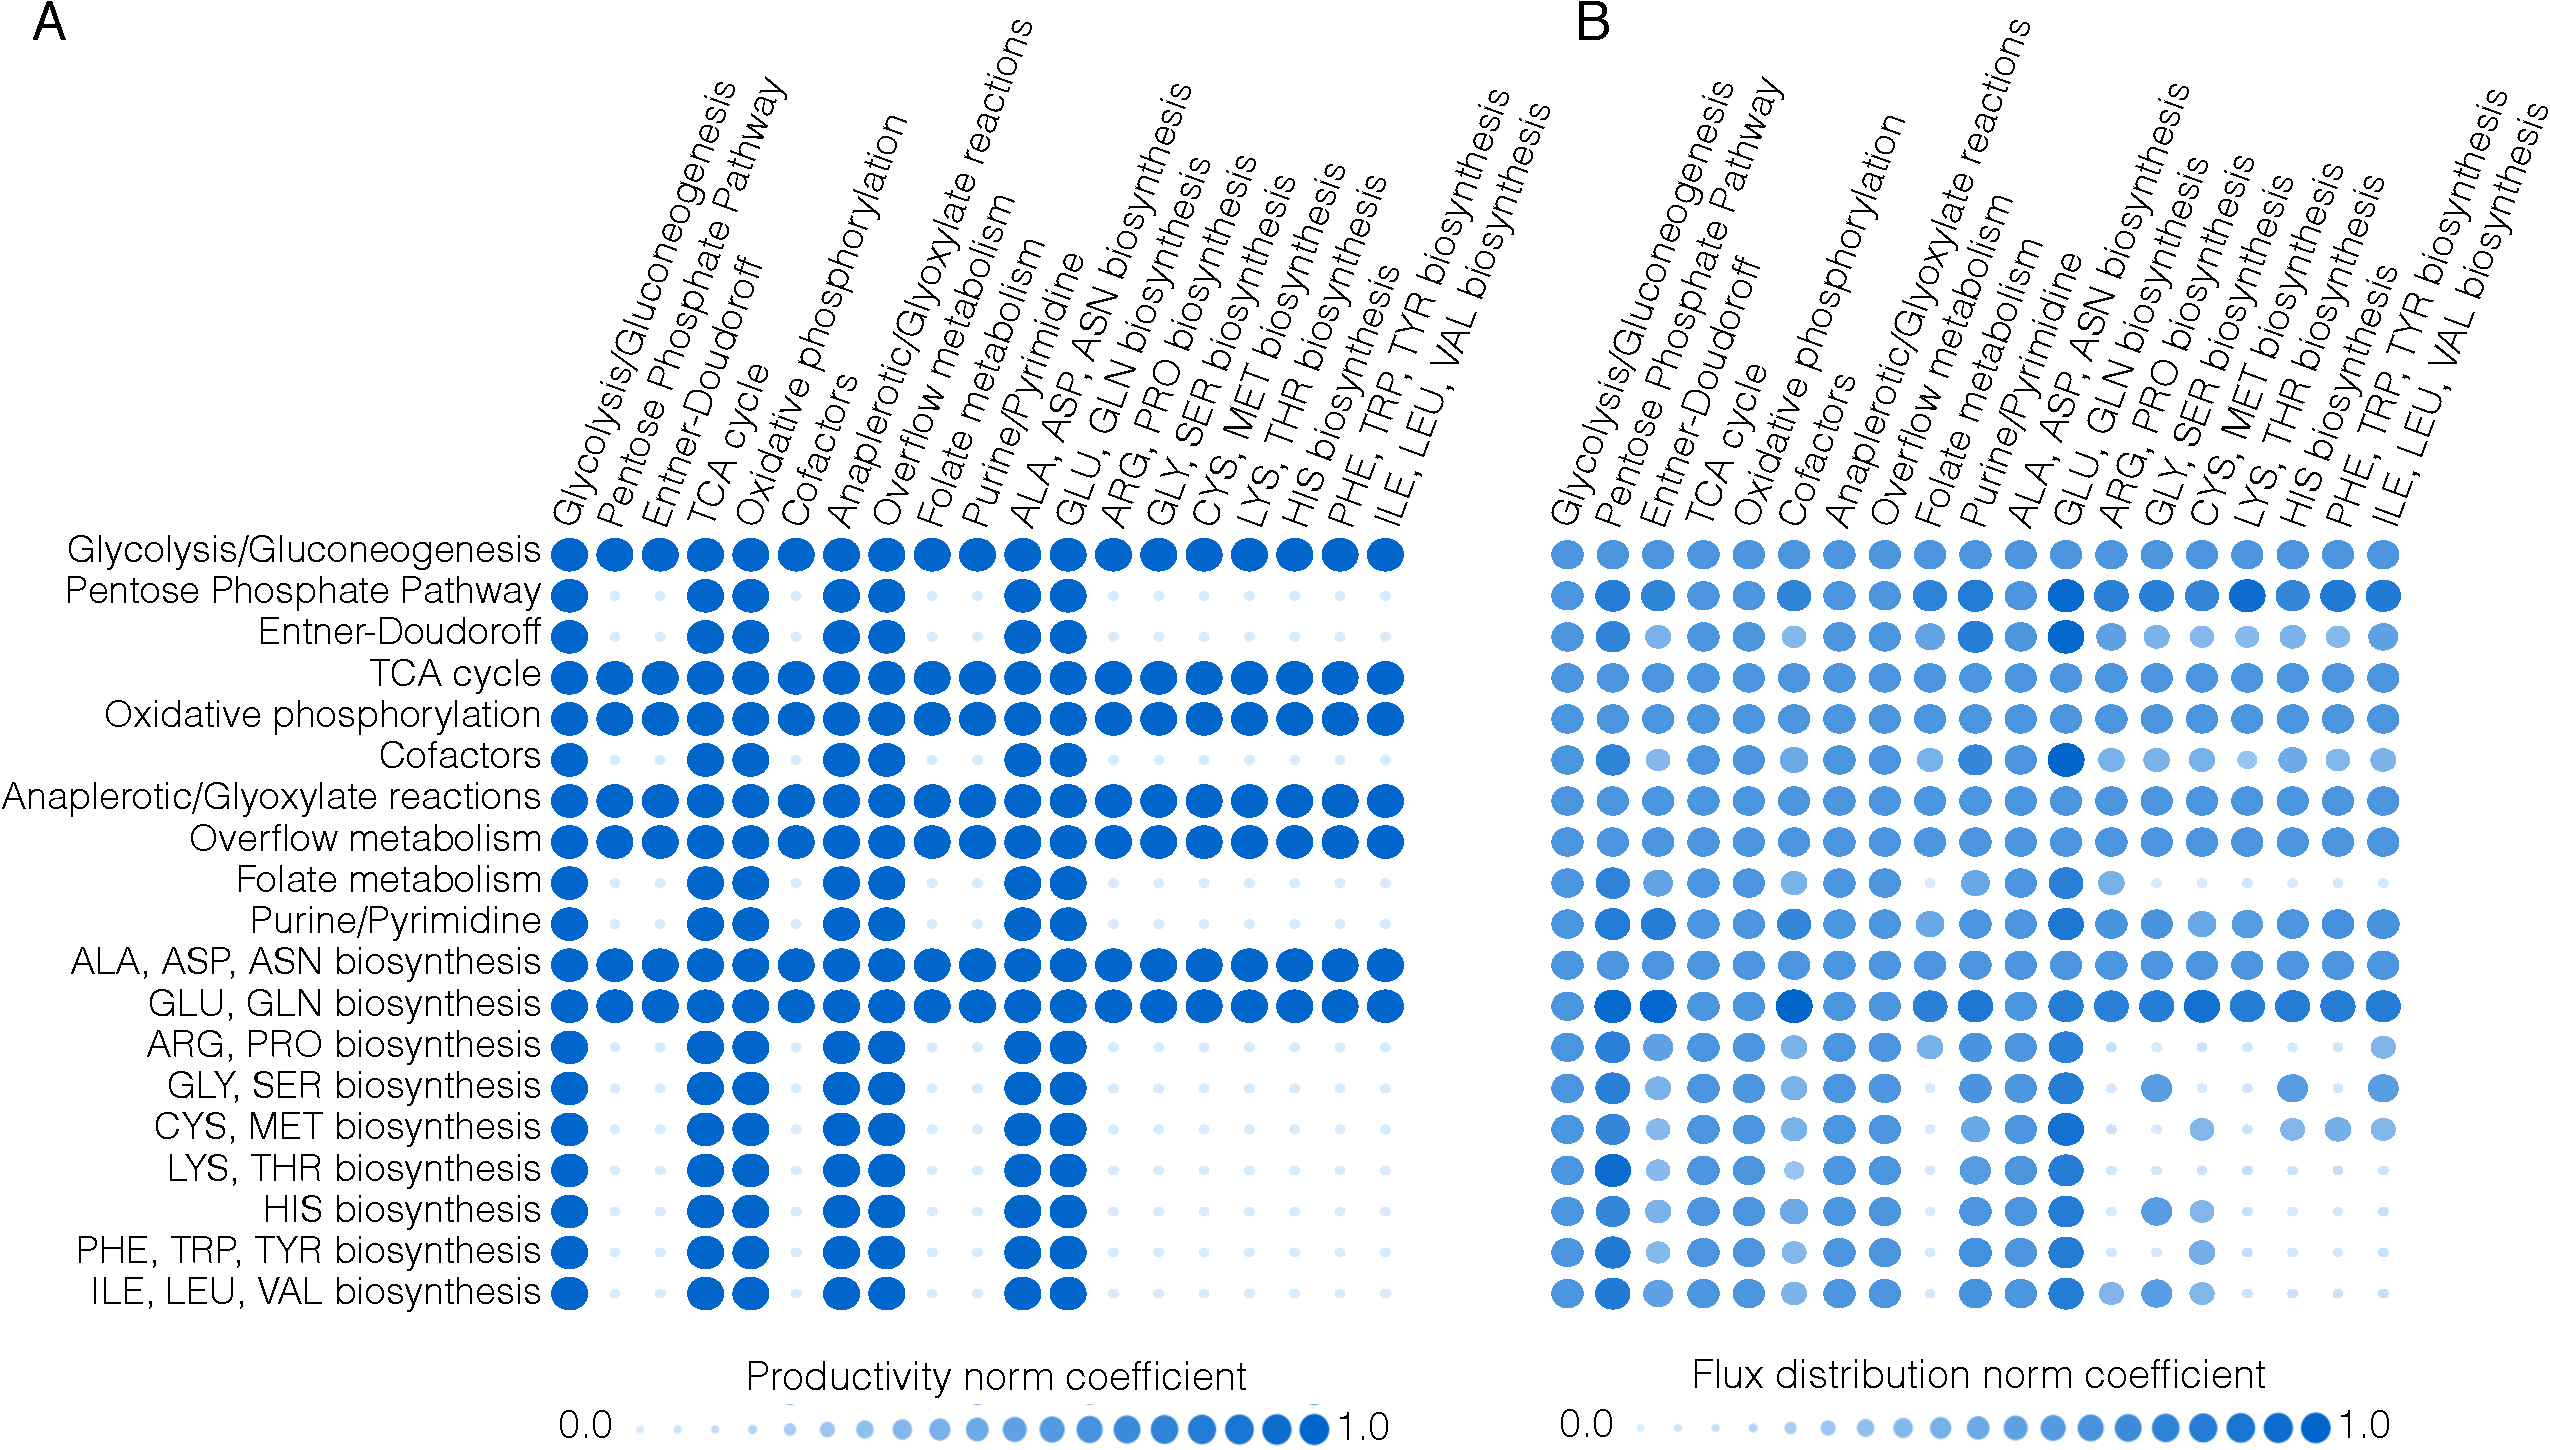
\includegraphics[width=1.0\textwidth]{./figs/Fig-7-FluxDistribution-Analysis.pdf}
\caption{The norm effect of pairwise knockouts of subgroups in the cell-free network (A) CAT productivity norm compared to no knockouts in the experimentally constrained case. (B) Flux distribution norm compared to no knockouts in the experimentally constrained case.}
\label{fig:norm}
\end{figure}

% Despite the constraints by experimental measurements, it is difficult to calculate the physiological flux distribution of metabolism (Fig.~\ref{fig:norm})
% For example, there is a high flux through the Entner-Douodoroff pathway, but this may be an artifact of the optimal solution.
% Flux balance analysis has been shown to have multiple alternative optimal solutions with flux variablitiy analysis and mixed-integer linear programming resulting in a poor depiction of the physiological flux distribution \cite{LEE2000711, Mahadevan2003264, Schuetz119}.


\subsection{Summary and conclusions}
In this study, we developed a sequence specific constraint based modeling approach to predict the performance of cell-free protein synthesis reactions for a range of proteins. We showed first principle predictions for protein production of deGFP and CAT which were in agreement with experimental measurements, under two different promoters and two different cell-free extract systems.
We are currently working on expanding our library of promoters that can provide good estimates of performance for different proteins.
Different promoter will help design \emph{de~novo} circuits for optimal functionality and performance.
This modeling approach suggested correlations for productivity, energy efficiency and carbon yield as a function of the size of the protein.
Maltose binding protein showed good agreement with these performance metrics with the established model correlations.
Furthermore, global sensitivity analysis identified oxygen uptake as being instrumental for maintaining a high energy efficiency and carbon yield.
The translation rate was identified as the rate limiting step for productivity.
The model also suggested that cell-free systems can simultaneously operate aerobically and anaerobically, which can lead to inefficient production and should be addressed to optimize energy efficiency and carbon yield.
In addition, our modeling approach could be expanded with a more detailed description of gene expression that has been utilized in a \emph{E. coli} genome scale model \cite{Brien693}.
We would also like to expand our model to include post translation modifications that proteins would require for proper folding and functionality.
In conclusion, sequence specific constraint based modeling offers a novel means to \emph{a~priori} estimate the performance of cell-free synthetic circuits.

\clearpage

\section*{Materials and Methods}

\subsection*{Glucose/NMP cell-free protein synthesis.}
The glucose/NMP cell-free protein synthesis reaction was
performed using the S30 extract in 1.5-mL Eppendorf tubes (working volume of 15 $\mu$L) and incubated in a humidified incubator.
The S30 extract was prepared from \textit{E.~coli} strain KC6 (A19 $\Delta$tonA $\Delta$tnaA $\Delta$speA $\Delta$endA $\Delta$sdaA $\Delta$sdaB $\Delta$gshA met+).
This K12-derivative has several gene deletions to stabilize amino acid concentrations during the cell-free reaction.
The KC6 strain was grown to approximately 3.0 OD595 in a 10-L fermenter (B. Braun, Allentown PA) on defined media with glucose as the carbon source and with the addition of 13 amino acids (alanine, arginine, cysteine, serine, aspartate, glutamate, and glutamine were excluded) \cite{Zawada:2003}. Crude S30 extract was prepared as described previously \cite{Jewett:2002}.
Plasmid pK7CAT was used as the DNA template for chloramphenical acetyl transferase (CAT) expression by placing the \emph{cat} gene
between the T7 promoter and the T7 terminator \cite{Kigawa1995}.
The plasmid was isolated and purified using a Plasmid Maxi Kit (Qiagen, Valencia CA).
Cell-free CAT synthesis was performed at 37 $^{\circ}$C.

The protein synthesis reaction was conducted using the PANOxSP protocol with slight modifications from that described previously \cite{BIT:BIT20026}.
Unless otherwise noted, all reagents were purchased from Sigma (St. Louis, MO).
The initial mixture included 1.2 mM ATP; 0.85 mM each of GTP, UTP, and CTP; 30 mM phosphoenolpyruvate (Roche, Indianapolis IN); 130 mM potassium glutamate; 10 mM ammonium glutamate; 16 mM magnesium glutamate; 50 mM HEPES-KOH buffer (pH 7.5); 1.5 mM spermidine; 1.0 mM putrescine; 34 $\mu$g/mL folinic acid; 170.6 $\mu$g/mL \textit{E.~coli} tRNA mixture (Roche, Indianapolis IN); 13.3 $\mu$g/mL pK7CAT plasmid; 100 $\mu$g/mL T7 RNA polymerase; 20 unlabeled amino acids at 2-3 mM each; 5 $\mu$M l-[U-\textsuperscript{14}C]-leucine (Amersham Pharmacia, Uppsala Sweden); 0.33 mM nicotinamide adenine dinucleotide (NAD); 0.26 mM coenzyme A (CoA); 2.7 mM sodium oxalate; and 0.24 volumes of \textit{E.~coli} S30 extract.
This reaction was modified for the energy source used such that glucose reactions have 30-40 mM glucose in place of PEP.
Sodium oxalate was not added since it has a detrimental effect on protein synthesis and ATP concentrations when using glucose or other early glycolytic intermediate energy sources \cite{BIT:BIT1121}. The HEPES buffer (pKa $\sim$ 7.5) was replaced with Bis-Tris (pKa $\sim$ 6.5). In addition, the magnesium glutamate concentration was reduced to 8 mM for the glucose reaction since a lower magnesium optimum was found when using a nonphosphorylated energy source \cite{BIT:BIT20026}. Finally, 10 mM phosphate was added in the form of potassium phosphate dibasic adjusted to pH 7.2 with acetic acid.

\subsection*{Protein product and metabolite measurements.}
Cell-free reaction samples were quenched at specific timepoints with equal volumes of ice-cold 150 mM sulfuric acid to precipitate proteins.
Protein synthesis of CAT was determined from the total amount of \textsuperscript{14}C-leucine-labeled product by trichloroacetic acid precipitation followed by scintillation counting as described previously \cite{2005_calhoun_BiotechnologyProgress}.
Samples were centrifuged for 10 min at 12,000g and 4$^{\circ}$C.
The supernatant was collected for high performance liquid chromatography (HPLC) analysis.
HPLC analysis (Agilent 1100 HPLC, Palo Alto CA) was used to separate nucleotides and organic acids, including glucose. Compounds were identified and quantified by comparison to known standards for retention time and UV absorbance (260 nm for nucleotides and 210 nm for organic acids) as described previously \cite{2005_calhoun_BiotechnologyProgress}.
The standard compounds quantified with a refractive index detector included inorganic phosphate, glucose, and acetate.
Pyruvate, malate, succinate, and lactate were quantified with the UV detector.
The stability of the amino acids in the cell extract was determined using a Dionex Amino Acid Analysis (AAA) HPLC System (Sunnyvale, CA) that separates amino acids by gradient anion exchange (AminoPac PA10 column).
Compounds were identified with pulsed amperometric electrochemical detection and by comparison to known standards.

\subsection*{Formulation and solution of the model equations.}
The sequence-specific flux balance analysis problem was formulated as a linear program:
\begin{equation}
 \begin{multlined}
	\qquad \qquad \qquad \max_{\boldsymbol{w}}{} \! \left( w_{X} = \mathbf{\boldsymbol{\theta}}^T \boldsymbol{w} \right) \\
	\mathrm{Subject \; to:}
	 \; \; \mathbf{S}\mathbf{w}=\mathbf{0} \\
\mathcal{L}_{i} \leq w_i \leq \mathcal{U}_{i}  \qquad i=1,2,\hdots,\mathcal{R}
 \end{multlined}
\end{equation}
where $\mathbf{S}$ denotes the stoichiometric matrix, $\mathbf{w}$ denotes the unknown flux vector, $\boldsymbol{\theta}$ denotes the objective cost vector
and $\mathcal{L}_{i}$ and $\mathcal{U}_{i}$ denote the lower and upper bounds on flux $w_{i}$, respectively.
The transcription (T) and translation (X) stoichiometry was modeled based upon the template reactions of Allen and Palsson \cite{Allen:2003aa}:
\begin{table}[!]
\centering
    \caption{Transcription and translation template reactions for protein production.}
    \renewcommand{\arraystretch}{1.2}
    \resizebox{\textwidth}{!}{\begin{tabular}{llcl} \toprule
        \textbf{Description} & \multicolumn{3}{l}{\textbf{Template reaction}} \\ \toprule
        Transcription initiation & $G_\mathcal{P}+R_{T}$ & $\longrightarrow$& $G_{\mathcal{P}}^{*}$ \\
        Transcription ($w_{T}$) & $G_{\mathcal{P}}^{*}+\quad\displaystyle\sum_{\mathclap{k\in\left\{A,C,G,U\right\}}}\eta_{k}\cdot \left(\left\{k\right\}TP + H_{2}O\right)$ & $\longrightarrow$& $mRNA+G_{\mathcal{P}}+R_{T}+\displaystyle\sum_{\mathclap{k\in\left\{A,C,G,U\right\}}} \eta_{k} \cdot PPi$ \\
        mRNA degradation &  $mRNA$ &$\longrightarrow$& \quad $\displaystyle\sum_{\mathclap{k\in\left\{A,C,G,U\right\}}}\eta_{k}\cdot \left\{k\right\}MP$ \\
	Translation initiation & $mRNA+R_{X}$ &$\longrightarrow$& $R_{X}^{*}$ \\
        tRNA charging & $\alpha_{j}\cdot \Big(AA_{j}+tRNA+ATP+H_{2}O\Big)$ &$\longrightarrow$& $\alpha_{j}\cdot \Big(AA_{j}\text{-}tRNA_{j} +AMP+PPi\Big)$ \\
 	&&& $\qquad \qquad \qquad \qquad \quad  {j=1,2,\hdots,20}$\\
        Translation ($w_{X}$) &  $R_{X}^{*}+\displaystyle\sum_{\mathclap{j\in\left\{AA\right\}}}\alpha_{j}\cdot \Big(AA_{j}\text{-} tRNA_{j}+2GTP+2H_{2}O\Big)$ &$\longrightarrow$& $\mathcal{P}+R_{X}+mRNA$\\
&&& $\quad +\displaystyle\sum_{\mathclap{j\in\left\{AA\right\}}}\alpha_{j}\cdot\Big(tRNA+2GDP+2Pi\Big)$ \\ \bottomrule
    \end{tabular}}
\label{tbl:parameters}
\end{table}
where $G_{\mathcal{P}}$ denotes the gene encoding protein product $\mathcal{P}$,
$R_{T}$ denotes the concentration of RNA polymerase,
$G_{\mathcal{P}}^{*}$ denotes the gene bounded by the RNA polymerase (open complex),
$\eta_{i}$ and $ \alpha_{j}$ denote the stoichiometric coefficients for nucleotide and amino acid, respectively,
$Pi$ denotes inorganic phosphate,
$R_{X}$ denotes the ribosome concentration,
$R_{X}^{*}$ denotes bound ribosome,
and $AA_{j}$ denotes $j^{th}$ amino acid.

The objective of the sequence specific flux balance calculation was to maximize the rate of protein translation, $w_{X}$.
The total glucose uptake rate was bounded by [0,40 mM/h] according to experimental data, while the amino acid uptake rates were bounded by [0,30 mM/h], but did not reach the maximum flux.
Gene and protein sequences were taken from literature and are available in the Supporting Information.
The sequence specific flux balance linear program was solved using the GNU Linear Programming Kit (GLPK) v4.55 \cite{GLPK}.
For all cases, amino acid degradation reactions were blocked as these enzymes were knocked out during the cell-free extract preparation \cite{2005_calhoun_BiotechnologyProgress, Garamella:2016aa}.
In the second case, all amino acid synthesis reactions were set to 0 mM/hr since \textit{E. coli} was grown in the presence of amino acids, thus these enzymes would not be present in the cell-free extract media.
In the third case, amino acid uptake reactions were set to 0 mM/hr.
In the experimental constrained case, \textit{E. coli} was grown in the presence of 13 amino acids (alanine, arginine, cysteine, serine, aspartate, glutamate, and glutamine were excluded) \cite{Zawada:2003}, thus the synthesis reactions responsible for those 13 amino acid were set to 0 mM/hr.


% We estimated the theoretical maximum performance of the cell-free protein synthesis system using sequence specific flux balance analysis (ssFBA) \cite{Allen:2003aa}.
% The sequence specific flux balance analysis problem was formulated as a linear program:
% \begin{equation}
%  \begin{multlined}
% 	\qquad \qquad \qquad \max_{\boldsymbol{w}}{} \! \left( w_{TL} = \mathbf{\boldsymbol{\theta}}^T \boldsymbol{w} \right) \\
% 	\mathrm{Subject \; to:}
% 	 \; \; \mathbf{S}\mathbf{w}=\mathbf{0} \\
% \alpha_i \leq w_i \leq \beta_i  \qquad i=1,2,\hdots,\mathcal{R}
%  \end{multlined}
% \end{equation}
% where $\mathbf{S}$ denotes the stoichiometric matrix, $\mathbf{w}$ denotes the unknown flux vector, $\boldsymbol{\theta}$ denotes the objective selection vector
% and $\alpha_i$ and $\beta_i$ denote the lower and upper bounds on flux $w_{i}$, respectively.
% The stoichiometry of the kinetic model was used for the ssFBA calculations, with the execpetion of the transcription and translation rates.
% The transcription (TX) and translation (TL) stoichiometry was modeled using the template reactions taken from Allen and Palsson \cite{Allen:2003aa}:
% \begin{eqnarray*}
% \mathrm{{G}_{\mathcal{P}}}+\mathrm{{R}_{1}} &\longrightarrow& \mathrm{G_{\mathcal{P}}^{*}} \\
% \mathrm{G_{\mathcal{P}}^{*}}+\sum_{\mathrm{k\in\left\{A,C,G,U\right\}}}\eta_{k}\cdot \mathrm{\left\{k\right\}TP} &\overset{\rm TX}{\longrightarrow}& \mathrm{mRNA}+\mathrm{G_{\mathcal{P}}}+\mathrm{R_{T}}+ \mathrm{\sum_{k\in\left\{A,C,G,U\right\}}2\eta_{k}\cdot Pi}\\
% \mathrm{mRNA} &\longrightarrow& \mathrm{\sum_{k\in\left\{A,C,G,U\right\}}\eta_{k}\cdot \left\{k\right\}MP} \\
% \mathrm{mRNA}+\mathrm{R_{X}} &\longrightarrow& \mathrm{R_{X}^{*}} \\
% \mathrm{\alpha_{j}\cdot AA_{j}+\alpha_{j}\cdot tRNA+\alpha_{j}\cdot ATP} &\longrightarrow& \mathrm{\alpha_{j}\cdot AA_{j}-tRNA_{j}+}\\
% && \mathrm{\qquad \alpha_{j}\cdot AMP+2\alpha_{j}\cdot Pi} \qquad{j=1,2,\hdots,20}\\
% \mathrm{R_{X}^{*}+\sum_{j\in\left\{AA\right\}}\alpha_{j}\cdot \Big(AA_{j}-tRNA_{j}+2\cdot GTP\Big)} &\stackrel{\rm TL}{\longrightarrow}& \mathcal{P}+\mathrm{R_{X}+mRNA}+\\
% && \mathrm{\quad +\sum_{j\in\left\{AA\right\}}\alpha_{j}\cdot\Big(tRNA+2\cdot GDP+2\cdot Pi\Big)}
% \end{eqnarray*}
% where $G_{\mathcal{P}}$ denotes the gene encoding protein product $\mathcal{P}$,
% $\rm R_{T}$ denotes the concentration of RNA polymerase,
% $G_{\mathcal{P}}^{*}$ denotes the gene bounded by the RNA polymerase,
% $\eta_{i}$ and $ \alpha_{j}$ denote the stoichiometric coefficients for nucleotide and amino acid, respectively,
% $\rm Pi$ denotes inorganic phosphate,
% $\rm R_{X}$ denotes the ribosome concentration,
% $\rm R_{X}^{*}$ denotes bounded ribosome,
% and $AA_{j}$ denotes the $j^{th}$ amino acid.

The bounds on the transcription rate ($\mathcal{L}_{T}=w_{T}=\mathcal{U}_{T}$) were modeled as:
\begin{equation}
	w_{T} = V_{T}^{max}\left(\frac{G_{\mathcal{P}}}{K_{T}+G_{\mathcal{P}}}\right)
\end{equation}
where $G_{\mathcal{P}}$ denotes the gene concentration of the protein of interest, and $K_{T}$ denotes a transcription saturation coefficient.
The maximum transcription rate $V_{T}^{max}$ was formulated as:
\begin{equation}
	V_{T}^{max} \equiv \left[R_{T}\left(\frac{\dot{v}_{T}}{l_{G}}\right)u\left(\kappa\right)\right]
\end{equation}
The term $R_{T}$ denotes the RNA polymerase concentration (nM),
$\dot{v}_{T}$ denotes the RNA polymerase elongation rate (nt/h),
$l_{G}$ denotes the gene length in nucleotides (nt).
The term $u\left(\kappa\right)$ (dimensionless, $0\leq u\left(\kappa\right)\leq 1$)
is an effective model of promoter activity, where $\kappa$ denotes promoter specific parameters.
The general form for the promoter models was taken from Moon $\emph{et~al.}$ \cite{Moon:2012ab}.
In this study, we considered two promoters: T7 and P70a.
The promoter function for the T7 promoter, $u_{T7}$, was given by:
\begin{equation}
	u_{T7} = \frac{K_{T7}}{1 + K_{T7}}
\end{equation}
where $K_{T7}$ denotes a T7 RNA polymerase binding constant.
The P70a promoter function $u_{P70a}$ (which was used for all other proteins) was formulated as:
\begin{equation}
	u_{P70a} = \frac{K_{1}+K_{2}f_{\sigma_{70}}}{1 + K_{1}+K_{2}f_{\sigma_{70}}}
\end{equation}
where $K_{1}$ denotes the weight of RNA polymerase binding alone,
$K_{2}$ denotes the weight of RNAP-$\sigma_{70}$ bound to the promoter,
and $f_{p70}$ denotes the fraction of the $\sigma_{70}$ transcription factor bound to RNAP, modeled as a Hill function:
\begin{equation}
	f_{\sigma_{70}} = \frac{\sigma_{70}^{n}}{K_{D}^{n} + \sigma_{70}^{n}}
\end{equation}
where $\sigma_{70}$ denotes the sigma-factor 70 concentration, $K_{D}$ denotes the dissociation constant, and $n$ denotes a cooperativity coefficient.
The values for all promoter parameters are given in Table ~\ref{tbl:parameters}.

The translation rate ($w_{X}$) was bounded by:
 \begin{equation}
	0\leq w_{X} \leq V_{X}^{max}\left(\frac{mRNA^{*}}{K_{X}+mRNA^{*}}\right)
\end{equation}
where $\rm mRNA^{*}$ denotes the steady state mRNA abundance and $K_{X}$ denotes a translation saturation constant.
The maximum translation rate $V_{X}^{max}$ was formulated as:
\begin{equation}
	V_{X}^{max} \equiv \left[K_{P} R_{X}\left(\frac{\dot{v}_{X}}{l_{P}}\right)\right]
\end{equation}
The term $K_{P}$ denotes the polysome amplification constant,
$\dot{v}_{X}$ denotes the ribosome elongation rate (amino acids per hour),
$l_{P}$ denotes the number of amino acids in the protein of interest.
The steady-state mRNA abundance $\rm mRNA^{*}$ was estimated as:
\begin{equation}
	 mRNA^{*}\simeq\frac{w_{T}}{\lambda}
\end{equation}
where $\lambda$ denotes the rate constant controlling the mRNA degradation rate (hr$^{-1}$).
All translation parameters are given in Table \ref{tbl:parameters}.

\begin{table}[!]
\centering
    \caption{Parameters for sequence specific flux balance analysis}
    \renewcommand{\arraystretch}{1}
    \begin{tabular}{lcccc} \toprule
        \textbf{Description} & \textbf{Parameter} & \textbf{Value} & \textbf{Units} & \textbf{Reference} \\ \toprule
        RNA polymerase concentration & $R_{T}$ & 75 & nM & \cite{Garamella:2016aa} \\
        Ribosome concentration & $R_{X}$ & 1.6 & $\mu$M & \cite{Garamella:2016aa, 2005_underwood_biotech} \\

        & & & & \\
        Transcription elongation rate & $\dot{v}_{T}$ & 25 & nt/sec & \cite{Garamella:2016aa} \\
        Translation elongation rate & $\dot{v}_{X}$ & 2 & aa/sec & \cite{Garamella:2016aa, 2005_underwood_biotech} \\
        Transcription saturation coefficient & $K_{T}$ & 3.5 & nM & estimated \\
        Translation saturation coefficient & $K_{X}$ & 45.0 & $\mu$M & estimated \\
        Polysome amplification constant & $K_{P}$ & 10 & constant & estimated \\
        mRNA degradation rate & $\lambda$ & 5.2 & hr\textsuperscript{-1} & \cite{Garamella:2016aa} \\

        & & & & \\
        T7 promoter & $K_{T7}$ & 10 & constant & estimated \\
        Weight RNA polymerase binding alone P70a & $K_{1}$ & 0.014 & constant & estimated \\
        Weight bound RNAP-$\sigma_{70}$ P70a & $K_{2}$ & 10 & constant & estimated \\
        $\sigma_{70}$ concentration & $\sigma_{70}$ & 35 & nM & \cite{Garamella:2016aa} \\
        $\sigma_{70}$ dissociation constant & $K_{D}$ & 130 & nM & \cite{Mauri2014} \\
	      $\sigma_{70}$ hill coefficient & n & 1 & constant & \cite{Mauri2014} \\
        Gene concentration & $G_{\mathcal{P}}$ & 5 & nM &  \cite{Garamella:2016aa} \\ \bottomrule

        % & & & & \\
	      %
        % Gene length of CAT & $l_{G}$ & 683 & nt & \cite{Kigawa1995} \\
        % Gene length of deGFP & $l_{G}$ & 660 & nt & \cite{Garamella:2016aa} \\
        % Protein length of CAT & $l_{P}$ & 229 & aa & \cite{Kigawa1995} \\
        % Protein length of deGFP & $l_{P}$ & 219 & aa & \cite{Garamella:2016aa} \\
    \end{tabular}
\label{tbl:parameters}
\end{table}

\clearpage

\subsection*{Calculation of energy efficiency.}
Energy efficiency ($\mathcal{E}$) was calculated as the ratio of protein production to glucose consumption, written in terms of equivalent ATP molecules:
\begin{equation}\label{eqn:energy-efficiency-definition}
	\mathcal{E}\equiv\Bigl(\frac{\texttt{q}_{POI}}{\texttt{q}_{GLC}\cdot\texttt{ATP}_{GLC}}\Bigr)\cdot \Bigl(2\times\left(\rm {ATP}_{T}+\rm {CTP}_{T}+\rm {GTP}_{T}+\rm {UTP}_{T}\right)+\rm2\cdot\rm {ATP}_{X}+\rm {GTP}_{X}\Bigl)
\end{equation}
where $\texttt{q}_{POI}=w_{X}$ denotes the production rate for the protein of interest, $\rm {ATP}_{X}$, $\rm {CTP}_{X}$, $\rm {GTP}_{X}$, $\rm {UTP}_{X}$ denote the stoichiometric coefficients of each energy species for the transcription of the protein of interest, $\rm {ATP}_{X}$, $\rm {GTP}_{X}$ denote the stoichiometric coefficients of ATP and GTP for the translation of the protein of interest, $\texttt{q}_{GLC}=w_{GLC}$ denotes the glucose uptake rate,
and $\texttt{ATP}_{GLC}$ denotes the equivalent ATP number for glucose.
The energy species stoichiometric coefficients are available in the Supporting Information.

\subsection*{Calculation of the carbon yield.}
The carbon yield ($Y_{C}^{POI}$) was calculated as the ratio of carbon produced as the protein of interest divided by the carbon consumed as reactants (glucose and amino acids):
\begin{equation}\label{eqn:yield-definition}
	Y_{C}^{POI}\equiv\frac{\texttt{q}_{POI}\cdot C_{POI}}{\displaystyle\sum_{i=1}^{\mathcal{R}} \texttt{q}_{m_{i}}\cdot C_{m_i}}
\end{equation}
where $\texttt{q}_{POI}$ denotes the flux of the protein of interest produced, $C_{POI}$ denotes carbon number of the protein of interest, $\mathcal{R}$ denotes the number of reactants,
$\texttt{q}_{m_{i}}$ denotes the uptake flux of the $i^{th}$ reactant, and $C_{m_i}$ denotes the carbon number of the $i^{th}$ reactant.


\subsection*{Quantification of uncertainty.}
Experimental factors taken from literature, for example macromolecular concentrations or elongation rates, have uncertainty associated with their values.
To quantify the influence of this uncertainty on model performance, we randomly sampled the expected physiological ranges for these parameters as determined from literature.
An ensemble of N = 100 flux distributions was calculated for the three different cases we considered:
control (with amino acid synthesis and uptake), amino acid uptake without synthesis, and amino acid synthesis without uptake.
The flux ensemble was calculated by randomly sampling the maximum glucose consumption rate within a range of 0 to 30 mM/h, (determined from experimental data)
and randomly sampling RNA polymerase levels, ribosome levels, and elongation rates in a physiological range determined from literature.
RNA polymerase levels were sampled between 60 and 80 nM, ribosome levels between 12 and 18 \textmu M, the RNA polymerase elongation rate between 20 and 30 nt/sec, and the ribosome elongation rate between 1.5 and 3 aa/s
\cite{2005_underwood_biotech, Garamella:2016aa}.

\subsection*{Global sensitivity analysis.}
We conducted a global sensitivity analysis using the variance-based method of Sobol to estimate which parameters controlled the performance of the cell-free protein synthesis reaction \citep{SOBOL_METHOD}.
We computed the total sensitivity index of each parameter relative to three performance objectives: productivity of the protein of interest, energy efficiency and carbon yield.
We established the sampling bounds for each parameter from literature.
We used the sampling method of Saltelli \textit{et al.} \citep{Saltelli:2010} to compute a family of $N\left(2d+2\right)$ parameter sets which obeyed our parameter ranges,
where $N$ was a parameter proportional to the desired number of model evaluations and $d$ was the number of parameters in the model. In our case, $N$ = 1000 and $d$ = 7, so the total sensitivity indices were computed from 16,000 model evaluations. The variance-based sensitivity analysis was conducted using the SALib module encoded in the Python programming language \citep{SALIB}.

\subsection*{Potential alternative optimal metabolic flux solutions.}
We identified potential alternative optimal metabolic flux distributions by performing single and pairwise reaction group knockout simulations [TODO:REF].
Reaction group knockouts were simulated by setting the flux bounds for all the reactions involved in a group to zero.
We grouped reactions in the cell-free network into 19 subgroups (available in Supporting Information).
We computed the difference ($l^{2}$-norm) for CAT productivity in the presence and absence of pairwise reaction knockouts.
Simultaneously, we computed the difference in the flux distribution ($l^{2}$-norm) for each pairwise reaction knockout compared to the flux distribution with no knockouts.
Those solutions with the same or similar productivity but large changes in the metabolic flux distribution represent alternative optimal soluations.

%%%%%%%%%%%%%%%%%%%%%%%%%%%%%%%%%%%%%%%%%%%%%%%%%%%%%%%%%%%%%%%%%%%%%
%% The "Acknowledgement" section can be given in all manuscript
%% classes.  This should be given within the "acknowledgement"
%% environment, which will make the correct section or running title.
%%%%%%%%%%%%%%%%%%%%%%%%%%%%%%%%%%%%%%%%%%%%%%%%%%%%%%%%%%%%%%%%%%%%%
\begin{acknowledgement}

This study was supported by an award from the US Army and Systems Biology of Trauma Induced Coagulopathy (W911NF-10-1-0376) to J.V. for the support of M.V.

\end{acknowledgement}

%%%%%%%%%%%%%%%%%%%%%%%%%%%%%%%%%%%%%%%%%%%%%%%%%%%%%%%%%%%%%%%%%%%%%
%% The same is true for Supporting Information, which should use the
%% suppinfo environment.
%%%%%%%%%%%%%%%%%%%%%%%%%%%%%%%%%%%%%%%%%%%%%%%%%%%%%%%%%%%%%%%%%%%%%
\begin{suppinfo}
The following files are available free of charge.
\begin{itemize}
  \item Protein Sequences: DNA and protein sequences of each protein of interest.
  \item Supporting Information: Performance trendlines as a function of carbon number, transcription/translation stoichiometric coefficients of energy species, and experimental measurements of CAT production.
  \item Carbon Yield Sensitivity Analysis: Global sensitivity analysis on deGFP carbon yield.
  \item Metabolites and reactions of the cell-free stoichiometric network.
\end{itemize}
\end{suppinfo}

\clearpage

%%%%%%%%%%%%%%%%%%%%%%%%%%%%%%%%%%%%%%%%%%%%%%%%%%%%%%%%%%%%%%%%%%%%%
%% The appropriate \bibliography command should be placed here.
%% Notice that the class file automatically sets \bibliographystyle
%% and also names the section correctly.
%%%%%%%%%%%%%%%%%%%%%%%%%%%%%%%%%%%%%%%%%%%%%%%%%%%%%%%%%%%%%%%%%%%%%
\bibliography{References_v1}

\end{document}
\grid
